\section{Mức độ 7,8 điểm}
\setcounter{dang}{0}
\setcounter{ex}{0}
\begin{dang}{Tính diện tích xung quanh, diện tích toàn phần, chiều cao, bán kính đáy. Thiết diện.}
\end{dang}
\Opensolutionfile{ans}[ans/CD22/Muc_7_8]
%%----1--9-D1---
\begin{ex}%[2H2K1-1]%Câu 1	(Mã 101-2021-Lần 2) 
	Cắt hình trụ $(T)$ bởi mặt phẳng song song với trục và cách trục một khoảng bằng $ 2a$, ta được thiết diện là một hình vuông có diện tích bằng $ 36a^2$. Diện tích xung quanh của $(T)$ bằng
	\choice
	{$ 4\sqrt{13}\pi a^2$}
	{\True $ 12\sqrt{13}\pi{a^2}$}
	{$ 6\sqrt{13}\pi a^2$}
	{$ 8\sqrt{13}\pi a^2$}
	\loigiai{
\begin{center}
\begin{tikzpicture}[scale=.9,font=\scriptsize]
	\draw (0,0) ellipse (2cm and 0.6cm);
	\draw (-2,0) -- (-2,-4);
	\draw (2,0) -- (2,-4);
	\draw (-2,-4) arc (180:360:2cm and 0.6cm);
	\draw[dashed] (2,-4) arc (0:180:2cm and 0.6cm);
	\fill (0,0) circle (1.5pt);
	\fill (0,-4) circle (1.5pt);
	\node[draw,fill,circle,inner sep=1pt,label={-100:$D$}] (D) at (-70:2cm and 0.6cm) {};
	\node[draw,fill,circle,inner sep=1pt,label={90:$C$}] (C) at (45:2cm and 0.6cm) {};
	\node[draw,fill,circle,inner sep=1pt,label={-90:$A$}] at ($(0,-4)+(-70:2 and 0.6)$) {};
	\node[draw,fill,circle,inner sep=1pt,label={30:$B$}] at ($(0,-4)+(45:2 and 0.6)$) {};
	\draw (-70:2cm and 0.6cm) -- ($(0,-4)+(-70:2 and 0.6)$);
	\draw (-70:2cm and 0.6cm) -- (45:2cm and 0.6cm);
	\draw[dashed] ($(0,-4)+(-70:2 and 0.6)$) -- ($(0,-4)+(45:2 and 0.6)$) -- (45:2cm and 0.6cm);
	\node[above] at (0,0) {O};
	\node[below] at (0,-4) {O'};
	\fill (2,0) circle (1.5pt);
	\coordinate (I) at ($(D)!0.5!(C)$);
	\node[draw,fill,circle,inner sep=1pt,label={90:$I$}] at (I) {};
	\draw (D) -- (0,0) -- (I);
\end{tikzpicture}
\end{center}
		Cắt hình trụ $(T)$ bởi mặt phẳng song song với trục $O{O}'$ ta được thiết diện là một hình vuông $ABCD$ có diện tích bằng $ 36a^2$. Suy ra $S_{ABCD}=C{D^2}=36a^2\Rightarrow CD=AD=6a$ .\\
		Gọi $ I$ là trung điểm của $ CD$, ta có:\\
		$\left\{\begin{aligned}
		& OI\perp CD\\ 
		& OI\perp AD\\ 
		\end{aligned}\right.\Rightarrow OI\perp\left(ABCD\right)\Rightarrow OI=d\left(O,\left(ABCD\right)\right)=d\left(O{O}',\left(ABCD\right)\right)=2a$.\\
		$\Delta OID$vuông tại $ I$ có $ ID=\dfrac{CD}{2}=3a;OI=2a\Rightarrow O{D^2}=O{I^2}+I{D^2}=13a^2\Rightarrow OD=a\sqrt{13}$.\\
		Suy ra $ r=OD=a\sqrt{13}$.\\
		Diện tích xung quanh của hình trụ $(T)$ là $S_{xq}=2\pi rl=2\pi  .a\sqrt{13}.6a=12\sqrt{13}\pi{a^2}$.}
\end{ex}

\begin{ex}%[2H2K1-1]%Câu 2	(Mã 102-2021-Lần 2) 
	Cắt hình trụ $(T)$ bởi mặt phẳng song song với trục và cách trục một khoảng bằng $ 3a$, ta được thiết diện là một hình vuông có diện tích bằng $ 16a^2$. Diện tích xung quanh của $(T)$ bằng
	\choice
	{$\dfrac{16\sqrt{13}}{3}\pi{a^2}$}
	{$ 4\sqrt{13}\pi{a^2}$}
	{$\dfrac{8\sqrt{13}}{3}\pi{a^2}$}
	{\True $ 8\sqrt{13}\pi{a^2}$}
	\loigiai{
\begin{center}
	\begin{tikzpicture}[scale=.9,font=\scriptsize]
	\draw (0,0) ellipse (2cm and 0.6cm);
	\draw (-2,0) -- (-2,-4);
	\draw (2,0) -- (2,-4);
	\draw (-2,-4) arc (180:360:2cm and 0.6cm);
	\draw[dashed] (2,-4) arc (0:180:2cm and 0.6cm);
	\fill (0,0) circle (1.5pt);
	\fill (0,-4) circle (1.5pt);
	\node[draw,fill,circle,inner sep=1pt,label={-100:$A$}] (A) at (-70:2cm and 0.6cm) {};
	\node[draw,fill,circle,inner sep=1pt,label={90:$B$}] (B) at (45:2cm and 0.6cm) {};
	\node[draw,fill,circle,inner sep=1pt,label={-90:$D$}] at ($(0,-4)+(-70:2 and 0.6)$) {};
	\node[draw,fill,circle,inner sep=1pt,label={30:$C$}] at ($(0,-4)+(45:2 and 0.6)$) {};
	\draw (-70:2cm and 0.6cm) -- ($(0,-4)+(-70:2 and 0.6)$);
	\draw (-70:2cm and 0.6cm) -- (45:2cm and 0.6cm);
	\draw[dashed] ($(0,-4)+(-70:2 and 0.6)$) -- ($(0,-4)+(45:2 and 0.6)$) -- (45:2cm and 0.6cm);
	\node[above] at (0,0) {O};
	\node[below] at (0,-4) {O'};
	\fill (2,0) circle (1.5pt);
	\coordinate (I) at ($(A)!0.5!(B)$);
	\node[draw,fill,circle,inner sep=1pt,label={90:$I$}] at (I) {};
	\draw (A) -- (0,0) -- (I);
\end{tikzpicture}
\end{center}	
		Gọi $(P)$ là mặt phẳng song song với trục $ O{O}'$.\\
		Theo giả thiết: Mặt phẳng $(P)$ cắt hình trụ $(T)$ theo thiết diện là hình vuông $ ABCD$.\\
		Khi đó, diện tích của hình vuông $S_{ABCD}=16a^2\Rightarrow AB=CD=4a$.\\
		Gọi $ I$là trung điểm $ AB\Rightarrow\left\{\begin{matrix}
		OI\perp AB\\
		OI\perp AD\\
		\end{matrix}\right.\Rightarrow OI\perp\left(ABCD\right)$. Do đó $ OI=3a$.\\
		Lại có: $ r=OA=\sqrt{O{I^2}+I{A^2}}=\sqrt{9a^2+4a^2}=a\sqrt{13}$.\\
		Diện tích xung quanh của hình trụ $(T)$ bằng: $S_{xq}=2\pi OA.AD=2\pi a\sqrt{13}.4a=8\sqrt{13}\pi{a^2}$.}
\end{ex}

\begin{ex}%[2H2K1-1]%Câu 3(Mã 111-2021-Lần 2) 
	Cắt hình trụ $(T)$ bởi mặt phẳng song song với trục và cách trục một khoảng bằng $ 2a$, ta được thiết diện là một hình vuông có diện tích bằng $ 16a^2$. Diện tích xung quanh của $(T)$ bằng
	\choice
	{$ 8\sqrt{2}\pi{a^2}$}
	{\True $ 16\sqrt{2}\pi{a^2}$}
	{$\dfrac{16\sqrt{2}}{3}\pi{a^2}$}
	{$\dfrac{32\sqrt{2}}{3}\pi{a^2}$}
	\loigiai{
\begin{center}
		\begin{tikzpicture}[scale=.9,font=\scriptsize]
	\draw (0,0) ellipse (2cm and 0.6cm);
	\draw (-2,0) -- (-2,-4);
	\draw (2,0) -- (2,-4);
	\draw (-2,-4) arc (180:360:2cm and 0.6cm);
	\draw[dashed] (2,-4) arc (0:180:2cm and 0.6cm);
	\fill (0,0) circle (1.5pt);
	\fill (0,-4) circle (1.5pt);
	\node[draw,fill,circle,inner sep=1pt,label={-100:$A$}] (A) at (-70:2cm and 0.6cm) {};
	\node[draw,fill,circle,inner sep=1pt,label={90:$B$}] (B) at (45:2cm and 0.6cm) {};
	\node[draw,fill,circle,inner sep=1pt,label={-90:$D$}] at ($(0,-4)+(-70:2 and 0.6)$) {};
	\node[draw,fill,circle,inner sep=1pt,label={30:$C$}] at ($(0,-4)+(45:2 and 0.6)$) {};
	\draw (-70:2cm and 0.6cm) -- ($(0,-4)+(-70:2 and 0.6)$);
	\draw (-70:2cm and 0.6cm) -- (45:2cm and 0.6cm);
	\draw[dashed] ($(0,-4)+(-70:2 and 0.6)$) -- ($(0,-4)+(45:2 and 0.6)$) -- (45:2cm and 0.6cm);
	\node[above] at (0,0) {O};
	\node[below] at (0,-4) {O'};
	\fill (2,0) circle (1.5pt);
	\coordinate (I) at ($(A)!0.5!(B)$);
	\node[draw,fill,circle,inner sep=1pt,label={90:$I$}] at (I) {};
	\draw (A) -- (0,0) -- (I);\
	%\draw (O) -- (0,0) -- (B);
\end{tikzpicture}
\end{center}
		Gọi thiết diện là hình vuông $ AB{B}'{A}'$ ; $ O,\text{O}'$ lần lượt là tâm của hai đáy, $ I$ là trung điểm $ AB$.\\
		Theo bài ra ta có: $ OI=2a$ và $S_{AB{B}'{A}'}=A{B^2}=16a^2$$\Leftrightarrow AB=4a$$\Rightarrow IA=\dfrac{1}{2}AB=2a$ và $ O{O}'=A{A}'=AB=4a$.\\
		Khi đó $ R=OA=\sqrt{A{I^2}+O{I^2}}=2\sqrt{2}a$.\\
		Vậy $S_{xq}=2\pi .R.h$$=2\pi .2\sqrt{2}a.4a$$=16\sqrt{2}\pi{a^2}$.}
\end{ex}

\begin{ex}%[2H2K1-1]%Câu 4(Mã 120-2021-Lần 2) 
	Cắt hình trụ $(T)$ bởi mặt phẳng song song với trục và cách trục một khoảng bằng $ 3a$, ta được thiết diện là một hình vuông có diện tích bằng $ 36a^2$. Diện tích xung quanh của $(T)$ bằng
	\choice
	{$ 24\sqrt{2}\pi{a^2}$}
	{$ 18\sqrt{2}\pi{a^2}$}
	{$ 12\sqrt{2}\pi{a^2}$}
	{\True $ 36\sqrt{2}\pi{a^2}$}
	\loigiai{
\begin{center}
	\begin{tikzpicture}[scale=.9,font=\scriptsize]
	\draw (0,0) ellipse (2cm and 0.6cm);
	\draw (-2,0) -- (-2,-4);
	\draw (2,0) -- (2,-4);
	\draw (-2,-4) arc (180:360:2cm and 0.6cm);
	\draw[dashed] (2,-4) arc (0:180:2cm and 0.6cm);
	\fill (0,0) circle (1.5pt);
	\fill (0,-4) circle (1.5pt);
	\node[draw,fill,circle,inner sep=1pt,label={-100:$A$}] (A) at (-70:2cm and 0.6cm) {};
	\node[draw,fill,circle,inner sep=1pt,label={90:$B$}] (B) at (45:2cm and 0.6cm) {};
	\node[draw,fill,circle,inner sep=1pt,label={-90:$D$}] at ($(0,-4)+(-70:2 and 0.6)$) {};
	\node[draw,fill,circle,inner sep=1pt,label={30:$C$}] at ($(0,-4)+(45:2 and 0.6)$) {};
	\draw (-70:2cm and 0.6cm) -- ($(0,-4)+(-70:2 and 0.6)$);
	\draw (-70:2cm and 0.6cm) -- (45:2cm and 0.6cm);
	\draw[dashed] ($(0,-4)+(-70:2 and 0.6)$) -- ($(0,-4)+(45:2 and 0.6)$) -- (45:2cm and 0.6cm);
	\node[above] at (0,0) {O};
	\node[below] at (0,-4) {O'};
	\fill (2,0) circle (1.5pt);
	\coordinate (I) at ($(A)!0.5!(B)$);
	\node[draw,fill,circle,inner sep=1pt,label={90:$I$}] at (I) {};
	\draw (A) -- (0,0) -- (I);
\end{tikzpicture}
\end{center}
		Gọi $ O,\,O'$ lần lượt là tâm hai mặt đáy của hình trụ, mặt phẳng cắt hình trụ theo thiết diện là hình vuông $ ABCD$.\\
		Diện tích hình vuông $ ABCD$ bằng $ 36a^2$ nên $ A{B^2}=A{D^2}=36a^2\Rightarrow AB=AD=6a$.\\
		Gọi $ I$ là trung điểm của $ AB$.\\
		Mặt phẳng song song với trục cách trục một khoảng bằng $ 3a$ nên $ OI=3a$.\\
		Tam giác $ AIO$ vuông tại $ I$ nên $ OA=\sqrt{O{I^2}+I{A^2}}$$=\sqrt{O{I^2}+\left(\dfrac{AB}{2}\right)^2}=\sqrt{\left(3a\right)^3+\left(3a\right)^3}=3a\sqrt{2}$.\\
		Mặt phẳng thiết diện song song với trục nên $ AD=O{O}'=6a$.\\
		Diện tích xung quanh của hình trụ $(T)$ là $S_{xq}=2.\pi .OA\text{O}{O}'=2.\pi .3a\sqrt{2}.6a$$=36\sqrt{2}\pi{a^2}$.}
\end{ex}

\begin{ex}%[2H2K1-1]%Câu 5(Mã 103-2019) 
	Cho hình trụ có chiều cao bằng $3\sqrt{2}$ . Cắt hình trụ đã cho bởi mặt phẳng song song với trục và cách trục một khoảng bằng 1, thiết diện thu được có diện tích bằng $12\sqrt{2}$ . Diện tích xung quanh của hình trụ đã cho bằng
	\choice
	{\True$ 6\sqrt{10}\pi $}
	{$ 6\sqrt{34}\pi $}
	{$ 3\sqrt{10}\pi $}
	{$ 3\sqrt{34}\pi $}
	\loigiai{
\immini{		Ta có:\\
	$\begin{aligned}
		&{S_{ABCD}}=12\sqrt{2}=3\sqrt{2}.CD\\ 
		&\Rightarrow CD=4\\ 
		&\Rightarrow CI=2\\ 
		&\Rightarrow CO=\sqrt{C{I^2}+I{O^2}}=\sqrt{5}=r\\ 
		&{S_{xq}}=2\pi rl=6\sqrt{10}\pi\\ 
	\end{aligned}$.}{\begin{tikzpicture}[scale=.9,font=\scriptsize]
		\draw (0,0) ellipse (2cm and 0.6cm);
		\draw (-2,0) -- (-2,-4);
		\draw (2,0) -- (2,-4);
		\draw (-2,-4) arc (180:360:2cm and 0.6cm);
		\draw[dashed] (2,-4) arc (0:180:2cm and 0.6cm);
		\fill (0,0) circle (1.5pt);
		\fill (0,-4) circle (1.5pt);
		\node[draw,fill,circle,inner sep=1pt,label={-100:$D$}] (D) at (-70:2cm and 0.6cm) {};
		\node[draw,fill,circle,inner sep=1pt,label={90:$C$}] (C) at (45:2cm and 0.6cm) {};
		\node[draw,fill,circle,inner sep=1pt,label={-90:$A$}] at ($(0,-4)+(-70:2 and 0.6)$) {};
		\node[draw,fill,circle,inner sep=1pt,label={30:$B$}] at ($(0,-4)+(45:2 and 0.6)$) {};
		\draw (-70:2cm and 0.6cm) -- ($(0,-4)+(-70:2 and 0.6)$);
		\draw (-70:2cm and 0.6cm) -- (45:2cm and 0.6cm);
		\draw[dashed] ($(0,-4)+(-70:2 and 0.6)$) -- ($(0,-4)+(45:2 and 0.6)$) -- (45:2cm and 0.6cm);
		\node[above] at (0,0) {O};
		\node[below] at (0,-4) {O'};
		\fill (2,0) circle (1.5pt);
		\coordinate (I) at ($(D)!0.5!(C)$);
		\node[draw,fill,circle,inner sep=1pt,label={90:$I$}] at (I) {};
		\draw (D) -- (0,0) -- (I);
	\end{tikzpicture}
}
}
\end{ex}

\begin{ex}%[2H2K1-1]%Câu 6(Mã 101-2019) 
	Cho hình trụ có chiều cao bằng $ 5\sqrt{3}$. Cắt hình trụ đã cho bởi mặt phẳng song song với trục và cách trục một khoảng bằng $ 1$, thiết diện thu được có diện tích bằng $ 30$. Diện tích xung quanh của hình trụ đã cho bằng
	\choice
	{$ 10\sqrt{3}\pi $}
	{$ 5\sqrt{39}\pi $}
	{\True$ 20\sqrt{3}\pi $}
	{$ 10\sqrt{39}\pi $}
	\loigiai{
	\begin{center}
	\begin{tikzpicture}[scale=.9,font=\scriptsize]
	\draw (0,0) ellipse (2cm and 0.6cm);
	\draw (-2,0) -- (-2,-4);
	\draw (2,0) -- (2,-4);
	\draw (-2,-4) arc (180:360:2cm and 0.6cm);
	\draw[dashed] (2,-4) arc (0:180:2cm and 0.6cm);
	\fill (0,0) circle (1.5pt);
	\fill (0,-4) circle (1.5pt);
	\node[draw,fill,circle,inner sep=1pt,label={-100:$A$}] (A) at (-70:2cm and 0.6cm) {};
	\node[draw,fill,circle,inner sep=1pt,label={90:$B$}] (B) at (45:2cm and 0.6cm) {};
	\node[draw,fill,circle,inner sep=1pt,label={-90:$D$}] at ($(0,-4)+(-70:2 and 0.6)$) {};
	\node[draw,fill,circle,inner sep=1pt,label={30:$C$}] at ($(0,-4)+(45:2 and 0.6)$) {};
	\draw (-70:2cm and 0.6cm) -- ($(0,-4)+(-70:2 and 0.6)$);
	\draw (-70:2cm and 0.6cm) -- (45:2cm and 0.6cm);
	\draw[dashed] ($(0,-4)+(-70:2 and 0.6)$) -- ($(0,-4)+(45:2 and 0.6)$) -- (45:2cm and 0.6cm);
	\node[above] at (0,0) {O};
	\node[below] at (0,-4) {O'};
	\fill (2,0) circle (1.5pt);
	\coordinate (H) at ($(A)!0.5!(B)$);
	\node[draw,fill,circle,inner sep=1pt,label={90:$H$}] at (H) {};
	\draw (A) -- (0,0) -- (H);
\end{tikzpicture}
	\end{center}
		Gọi $ O,\text{O}'$ lần lượt là tâm của hai đáy và $ ABCD$ là thiết diện song song với trục với $ A,B\in(O)$; $C,D\in\left(O'\right)$ . Gọi $ H$ là trung điểm của $ AB$$\Rightarrow OH=d\left(O{O}',\left(ABCD\right)\right)=1$.\\
		Vì $S_{ABCD}=30\Leftrightarrow AB.BC=30\Rightarrow AB=\dfrac{30}{5\sqrt{3}}=2\sqrt{3}\Rightarrow HA=HB=\sqrt{3}$.\\
		Bán kính của đáy là $ r=\sqrt{O{H^2}+H{A^2}}=\sqrt{3+1}=2$.\\
		Diện tích xung quanh của hình trụ bằng $S_{xq}=2\pi rh=2\pi .2.5\sqrt{3}=20\sqrt{3}\pi $.}
\end{ex}

\begin{ex}%[2H2K1-1]%Câu 7(Mã 102-2019) 
	Cho hình trụ có chiều cao bằng $ 4\sqrt{2}$. Cắt hình trụ đã cho bởi một mặt phẳng song song với trục và cách trục một khoảng bằng$\sqrt{2}$, thiết diện thu được có diện tích bằng $ 16$. Diện tích xung quanh của hình trụ đã cho bằng
	\choice
	{\True$ 16\sqrt{2}\pi $}
	{$ 8\sqrt{2}\pi $}
	{$ 12\sqrt{2}\pi $}
	{$ 24\sqrt{2}\pi $}
	\loigiai{
	\begin{center}
	\begin{tikzpicture}[scale=.9,font=\scriptsize]
	\draw (0,0) ellipse (2cm and 0.6cm);
	\draw (-2,0) -- (-2,-4);
	\draw (2,0) -- (2,-4);
	\draw (-2,-4) arc (180:360:2cm and 0.6cm);
	\draw[dashed] (2,-4) arc (0:180:2cm and 0.6cm);
	\fill (0,0) circle (1.5pt);
	\fill (0,-4) circle (1.5pt);
	\node[draw,fill,circle,inner sep=1pt,label={-100:$A$}] (A) at (-70:2cm and 0.6cm) {};
	\node[draw,fill,circle,inner sep=1pt,label={90:$B$}] (B) at (45:2cm and 0.6cm) {};
	\node[draw,fill,circle,inner sep=1pt,label={-90:$D$}] at ($(0,-4)+(-70:2 and 0.6)$) {};
	\node[draw,fill,circle,inner sep=1pt,label={30:$C$}] at ($(0,-4)+(45:2 and 0.6)$) {};
	\draw (-70:2cm and 0.6cm) -- ($(0,-4)+(-70:2 and 0.6)$);
	\draw (-70:2cm and 0.6cm) -- (45:2cm and 0.6cm);
	\draw[dashed] ($(0,-4)+(-70:2 and 0.6)$) -- ($(0,-4)+(45:2 and 0.6)$) -- (45:2cm and 0.6cm);
	\node[above] at (0,0) {O};
	\node[below] at (0,-4) {O'};
	\fill (2,0) circle (1.5pt);
	\coordinate (K) at ($(A)!0.5!(B)$);
	\node[draw,fill,circle,inner sep=1pt,label={90:$K$}] at (K) {};
	\draw (A) -- (0,0) -- (K);
\end{tikzpicture}
	\end{center}
		Cắt hình trụ đã cho bởi một mặt phẳng song song với trục, ta được thiết diện là hình chữ nhật $ ABCD$ (với $AB$ là dây cung của hình tròn đáy tâm $O$).\\
		Do hình trụ có chiều cao là $ h=O{O}'=4\sqrt{2}\Rightarrow $ hình trụ có độ dài đường sinh $ l=AD=4\sqrt{2}$.\\
		Diện tích hình chữ nhật $ ABCD$ bằng $ AB.CD=16$$\Rightarrow $$ AB=\dfrac{16}{AD}=\dfrac{16}{4\sqrt{2}}=2\sqrt{2}$.\\
		Gọi K là trung điểm đoạn $ AB$ thì $OK\perp AB$ , lại có$ mp(ABCD)$vuông góc với mặt phẳng đáy của hình trụ $\Rightarrow OK\perp mp(ABCD)\Rightarrow $ khoảng cách giữa  $ O{O}'$ và $ mp(ABCD)$ là $ OK=\sqrt{2}$.\\
		Xét tam giác vuông $ AOK$$ R=OA=\sqrt{O{K^2}+A{K^2}}=\sqrt{O{K^2}+\left(\dfrac{AB}{2}\right)^2}=\sqrt{\left(\sqrt{2}\right)^2+\left(\sqrt{2}\right)^2}=2$.\\
		Diện tích xung quanh của hình trụ là $ S=2\pi R.l=2\pi .2.4\sqrt{2}=16\pi\sqrt{2}$.}
\end{ex}

\begin{ex}%[2H2K1-1]%Câu 8
	Cắt hình trụ $(T)$ bằng một mặt phẳng đi qua trục được thiết diện là một hình chữ nhật có diện tích bằng $ 30\text{c}{\text{m}^{\text{2}}}$ và chu vi bằng $ 26\text{cm}$. Biết chiều dài của hình chữ nhật lớn hơn đường kính mặt đáy của hình trụ $(T)$. Diện tích toàn phần của $(T)$ là:
	\choice
	{$23\pi\left(\text{c}{\text{m}^{\text{2}}}\right)$}
	{$\dfrac{23\pi}{2}\left(\text{c}{\text{m}^2}\right)$}
	{\True $\dfrac{69\pi}{2}\left(\text{c}{\text{m}^2}\right)$}
	{$ 69\pi\left(\text{c}{\text{m}^2}\right)$}
	\loigiai{
	\begin{center}
		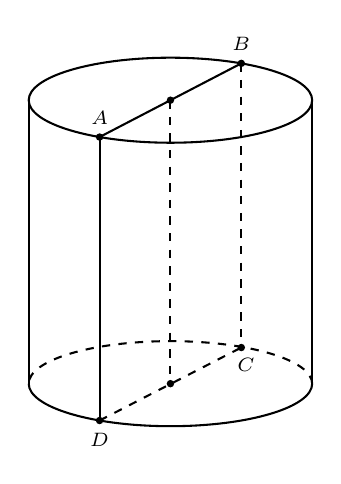
\begin{tikzpicture}[scale=.9,font=\scriptsize]
		\draw (0,0) ellipse (2cm and 0.6cm);
		\draw (-2,0) -- (-2,-4);
		\draw (2,0) -- (2,-4);
		\draw (-2,-4) arc (180:360:2cm and 0.6cm);
		\draw[dashed] (2,-4) arc (0:180:2cm and 0.6cm);
		%\node[left] at (0,0.2) {\normalsize$M$};
		\fill (0,0) circle (1.5pt);
		%\node[right] at (0,-4.1) {\normalsize$N$};
		\fill (0,-4) circle (1.5pt);
		\draw[dashed] (0,0) -- (0,-4);
		\fill (1,0.52) circle (1.5pt);
		\node at (-1,-0.25) {$A$};
		\fill (-1,-0.52) circle (1.5pt);
		\node at (1,0.8) {$B$};
		\draw (1,0.52) -- (-1,-0.52);
		\fill (1,-3.49) circle (1.5pt);
		\node[below right] at (0.8,-3.5) {$C$};
		\fill (-1,-4.52) circle (1.5pt);
		\node at (-1,-4.8) {$D$};
		\draw[dashed] (-1,-4.52) -- (1,-3.49);
		\draw[dashed] (1,0.52) -- (1,-3.49);
		\draw (-1,-0.52) -- (-1,-4.52);
	\end{tikzpicture}
	\end{center}
		Gọi $ h,r$ lần lượt là đường cao và bán kính đáy của hình trụ $(T)$. Thiết diện của mặt phẳng và hình trụ $(T)$ là hình chữ nhật $ ABCD$. Khi đó theo giả thiết ta có\\
		$\left\{\begin{aligned}
		& h>2r\\ 
		&{S_{ABCD}}=h.2r=30\\ 
		&{C_{ABCD}}=2(h+2r)=26\\ 
		\end{aligned}\right.\Leftrightarrow\left\{\begin{aligned}
		& h>2r\\ 
		& hr=15\\ 
		& h+2r=13\\ 
		\end{aligned}\right.\Leftrightarrow\left\{\begin{aligned}
		& h>2r\\ 
		& h=13-2r\\ 
		&-2r^2+15r-15=0\\ 
		\end{aligned}\right.\Leftrightarrow\left\{\begin{aligned}
		& h>2r\\ 
		& h=13-2r\\ 
		&\left[\begin{aligned}
		& r=5\Rightarrow h=3(l)\\ 
		& r=\dfrac{3}{2}\Rightarrow h=10(TM)\\ 
		\end{aligned}\right.\\ 
		\end{aligned}\right.$\\
		Vậy $S_{TP}=S_{XQ}+2S_=2\pi rh+2\pi{r^2}=2\pi .\dfrac{3}{2}.10+2\pi{\left(\dfrac{3}{2}\right)^2}=\dfrac{69\pi}{2}\left(\text{c}{\text{m}^2}\right)$.}
\end{ex}

\begin{ex}%[2H2K1-1]%Câu 9
	Một hình trụ có bán kính đáy bằng $50$ cm và có chiều cao là $50$ cm. Một đoạn thẳng $AB$ có chiều dài là $100$ cm và có hai đầu mút nằm trên hai đường tròn đáy. Tính khoảng cách $d$ từ đoạn thẳng đó đến trục hình trụ.
	\choice
	{$d=50$ cm}
	{$d=50\sqrt{3}$ cm}
	{\True $d=25$ cm}
	{$d=25\sqrt{3}$ cm}
	\loigiai{
\begin{center}
\begin{tikzpicture}
	\draw (0,0) ellipse (2cm and 0.6cm);
	\draw (-2,0) -- (-2,-4);
	\draw (2,0) -- (2,-4);
	\draw (-2,-4) arc (180:360:2cm and 0.6cm);
	\draw[dashed] (2,-4) arc (0:180:2cm and 0.6cm);
	\fill (0,0) circle (1.5pt);
	\fill (0,-4) circle (1.5pt);
	\node[draw,fill,circle,inner sep=1pt,label={90:$B$}] (B) at (+45:2cm and 0.6cm) {};
	\node[draw,fill,circle,inner sep=1pt,label={-90:$A$}] (A) at ($(0,-4)+(-70:2 and 0.6)$) {};
	\node[draw,fill,circle,inner sep=1pt,label={30:$C$}] (C) at ($(0,-4)+(45:2 and 0.6)$) {};
	\draw[dashed] (45:2cm and 0.6cm) -- ($(0,-4)+(45:2 and 0.6)$);
	\node[above] at (0,0) {$O'$};
	\node[below left] at (0,-4) {$O$};
	\coordinate (H) at ($(A)!0.5!(C)$);
	\draw[dashed] (A) --(0,-4)--(C)--(A) (0,-4)--(H) (0,0)--(0,-4) (A)--(B);
	\fill (H) circle (1.5pt);
	\node[right] at (H) {$H$};
\end{tikzpicture}
\end{center}
		Qua $ B$ kẻ đường thẳng song song với $O{O}'$ cắt đường tròn đáy tại $ C$.\\
		$ O{O}'\,\text{//}\,BC\Rightarrow O{O}'\,\text{//}\,\left(ABC\right)\Rightarrow d\left(O{O}',AB\right)=d\left(O{O}',\left(ABC\right)\right)=d\left(O,\left(ABC\right)\right)=OH=d$. ($ H$ là trung điểm của đoạn thẳng $ AC$).\\
		$ AC=\sqrt{A{B^2}-B{C^2}}=50\sqrt{3}$cm.\\
		Vậy $ d=OH=\sqrt{O{C^2}-H{C^2}}=25$cm.}
\end{ex}

%%---10-18--
\begin{ex}%[2H2K1-1]%Câu 10	(THPT Lê Quy Đôn Điện Biên 2019) 
	Một hình trụ tròn xoay có hai đáy là hai đường tròn $\left(O,R\right)$ và $\left(O',R\right)$. Biết rằng tồn tại dây cung $AB$ của đường tròn $\left(O,R\right)$sao cho tam giác $O'AB$ đều và góc giữa hai mặt phẳng $\left(O'AB\right)$ và mặt phẳng chứa đường tròn $\left(O,R\right)$ bằng $ 60^\circ $. Tính diện tích xung quanh của hình trụ đã cho.
	\choice
	{$ 4\pi{R^2}$}
	{$ 2\sqrt{3}\pi{R^2}$}
	{$\dfrac{3\sqrt{7}}{7}\pi{R^2}$}
	{\True $\dfrac{6\sqrt{7}}{7}\pi{R^2}$}
	\loigiai{
\begin{center}
	\begin{tikzpicture}
		\draw (0,0) ellipse (2cm and 0.6cm);
		\draw (-2,0) -- (-2,-4);
		\draw (2,0) -- (2,-4);
		\draw (-2,-4) arc (180:360:2cm and 0.6cm);
		\draw[dashed] (2,-4) arc (0:180:2cm and 0.6cm);
		\fill (0,0) circle (1.5pt);
		\fill (0,-4) circle (1.5pt);
		\node[draw,fill,circle,inner sep=1pt,label={-90:$A$}] (A) at ($(0,-4)+(-70:2 and 0.6)$) {};
		\node[draw,fill,circle,inner sep=1pt,label={-90:$A$}] (A) at ($(0,-4)+(-70:2 and 0.6)$) {};
		\node[draw,fill,circle,inner sep=1pt,label={30:$B$}] (B) at ($(0,-4)+(45:2 and 0.6)$) {};
		\node[above] at (0,0) {$O'$};
		\node[below left] at (0,-4) {$O$};
		\coordinate (K) at ($(A)!0.5!(B)$);
		\draw[dashed] (A) --(0,-4)--(B)--(A) (0,-4)--(K) (0,0)--(0,-4) (A)--(0,0)--(B);
		\fill (K) circle (1.5pt);
		\node[right] at (K) {$K$};
	\end{tikzpicture}	
\end{center}
		Gọi $ K$ là trung điểm $ AB$, đặt $ AB=2a$.\\
		Ta có : $ AB\perp OK$ và $ AB\perp O{O}'$ nên $\widehat{OK{O}'}=60^\circ $ $\Rightarrow{O}'K=2OK$ $\Rightarrow{O}'{K^2}=4O{K^2}$ $\Rightarrow 3a^2=4\left(R^2-a^2\right)$ $\Rightarrow{a^2}=\dfrac{4R^2}{7}$\\
		Mặt khác : $ O{O'^2}=O'{B^2}-O{B^2}=4a^2-R^2=4.\dfrac{4R^2}{7}-R^2=\dfrac{9R^2}{7}$ $\Rightarrow{O}'O=\dfrac{6\sqrt{7}\pi R}{7}$\\
		Vậy diện tích xung quanh hình trụ đã cho là : $S_{xq}=2\pi Rl=\dfrac{6\sqrt{7}\pi{R^2}}{7}$.}
\end{ex}

\begin{ex}%[2H2G1-1]%Câu 11(Chuyên Sơn La 2019) 
\immini{Cho khối trụ có bán kính đáy bằng $ 4\left(cm\right)$ và chiều cao $ 5\left(cm\right)$. Gọi $ AB$ là một dây cung đáy dưới sao cho $ AB=4\sqrt{3}\,\left(cm\right)$. Người ta dựng mặt phẳng $(P)$ đi qua hai điểm $ A$, $ B$ và tạo với mặt phẳng đáy hình trụ một góc $ 60^\circ$ như hình vẽ. Tính diện tích thiết diện của hình trụ cắt bởi mặt phẳng $(P)$.
	\choice
	{\True $\dfrac{8\left(4\pi-3\sqrt{3}\right)}{3}\,\left(c{m^2}\right)$}
	{$\dfrac{4\left(4\pi-\sqrt{3}\right)}{3}\,\left(c{m^2}\right)$}
	{$\dfrac{4\left(4\pi-3\sqrt{3}\right)}{3}\,\left(c{m^2}\right)$}
	{$\dfrac{8\left(4\pi-\sqrt{3}\right)}{3}\,\left(c{m^2}\right)$}}{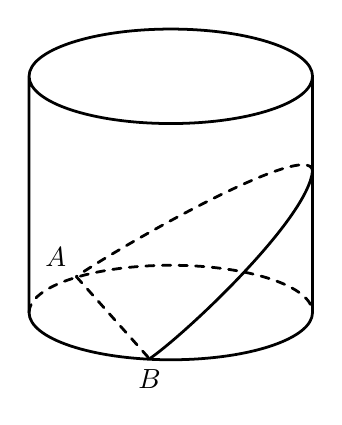
\begin{tikzpicture}[scale = 0.6, line join=round, line cap=round, >=stealth]
		
		\coordinate[] (O') at (0,6);
		\coordinate[] (O) at (0,0);
		\coordinate[] (C) at (3,0);
		\coordinate[label=above left:$A$] (A) at (-2,0.76);
		\coordinate[label=below:$B$] (B) at (-0.45,-0.98);
		\coordinate[] (D) at (-1.3,0);
		\coordinate[] (E) at (3,3);
		\def\a{3}
		\def\b{1}
		\def\h{5}
		
		\draw[dashed, line width = 1] (180:\a) arc
		(180:0:{\a} and {\b});
		\draw [thick, line width = 1] (-\a,\h)--(-\a,0) arc
		(180:360:{\a} and {\b})--(\a,\h)
		(90:\h) ellipse ({\a} and {\b});
		%	\draw[-,dashed, line width = 1] (O) -- (O');
		\draw[-,dashed,line width = 1] (A) -- (B);
		%	\draw[-,dashed,line width = 1] (C) -- (D);
		%	\draw[-,dashed, line width = 1] (D) -- (3,3);
		
		%	\fill[pattern= crosshatch dots] plot (C) arc
		%	(0:130:{\a} and {\b}) -- (A) -- (B) -- plot (B) arc
		%	(-99:0:{\a} and {\b}) ;
		
		\draw[line width = 1] (B)..controls+(35:1)and+(-95:1)..(3,3);
		\draw[dashed,line width = 1] (3,3)..controls+(95:0.7)and+(35:1)..(A);
		
		%	\begin{scope}% Kí hiệu góc
			%		\clip (E)--(D)--(C);
			%		\draw[line width = 1] (D) circle (1);
			%	\end{scope}
		
\end{tikzpicture}}
	\loigiai{
\begin{center}
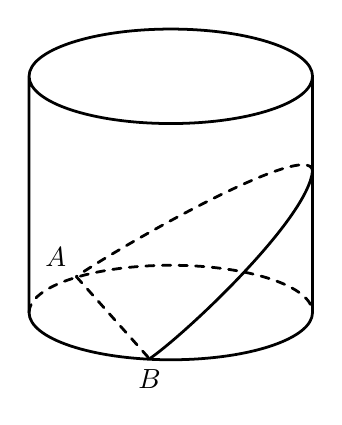
\begin{tikzpicture}[scale = 0.6, line join=round, line cap=round, >=stealth]
	
	\coordinate[] (O') at (0,6);
	\coordinate[] (O) at (0,0);
	\coordinate[] (C) at (3,0);
	\coordinate[label=above left:$A$] (A) at (-2,0.76);
	\coordinate[label=below:$B$] (B) at (-0.45,-0.98);
	\coordinate[] (D) at (-1.3,0);
	\coordinate[] (E) at (3,3);
	\def\a{3}
	\def\b{1}
	\def\h{5}
	
	\draw[dashed, line width = 1] (180:\a) arc
	(180:0:{\a} and {\b});
	\draw [thick, line width = 1] (-\a,\h)--(-\a,0) arc
	(180:360:{\a} and {\b})--(\a,\h)
	(90:\h) ellipse ({\a} and {\b});
	%	\draw[-,dashed, line width = 1] (O) -- (O');
	\draw[-,dashed,line width = 1] (A) -- (B);
	%	\draw[-,dashed,line width = 1] (C) -- (D);
	%	\draw[-,dashed, line width = 1] (D) -- (3,3);
	
	%	\fill[pattern= crosshatch dots] plot (C) arc
	%	(0:130:{\a} and {\b}) -- (A) -- (B) -- plot (B) arc
	%	(-99:0:{\a} and {\b}) ;
	
	\draw[line width = 1] (B)..controls+(35:1)and+(-95:1)..(3,3);
	\draw[dashed,line width = 1] (3,3)..controls+(95:0.7)and+(35:1)..(A);
	
	%	\begin{scope}% Kí hiệu góc
		%		\clip (E)--(D)--(C);
		%		\draw[line width = 1] (D) circle (1);
		%	\end{scope}
	
\end{tikzpicture}
\end{center}
		Gọi $ S$ là diện tích thiết diện, $S'$ là diện tích hình chiếu của thiết diện lên mặt phẳng\\
		đáy. Khi đó $S'=S.\cos 60^\circ $.\\
		Ta có $ AB=4\sqrt{3}\Rightarrow\cos\widehat{AOB}=\dfrac{O{A^2}+O{B^2}-A{B^2}}{2.OA.OB}=-\dfrac{1}{2}\Rightarrow\widehat{AOB}=120^\circ $\\
		$\left\{\begin{aligned}
		&{S_{OAB}}=\dfrac{1}{2}OA.OB.\sin 120^\circ=4\sqrt{3}\\ 
		&{S_{OAmB}}=\dfrac{1}{3}\pi .O{A^2}=\dfrac{16\pi}{3}\\ 
		\end{aligned}\right.\Rightarrow{S}'=S_{OAmB}-S_{OAB}=\dfrac{4\left(4\pi-3\sqrt{3}\right)}{3}$\\
		$ S=\dfrac{S'}{\cos 60^\circ}=\dfrac{8\left(4\pi-3\sqrt{3}\right)}{3}$.}
\end{ex}

\begin{ex}%Câu 12 [2H2B1-2]	[Toán Học Và Tuổi Trẻ 2018] 
	Cho hình lập phương có cạnh bằng $ 40$ $\text{cm}$ và một hình trụ có hai đáy là hai hình tròn nội tiếp hai mặt đối diện của hình lập phương. Gọi $S_1$, $S_2$ lần lượt là diện tích toàn phần của hình lập phương và diện tích toàn phần của hình trụ. Tính $ S=S_1+S_2$ $\left(\text{c}{\text{m}^2}\right)$.
	\choice
	{$ S=4\left(2400+\pi\right)$}
	{\True $ S=2400\left(4+\pi\right)$}
	{$ S=2400\left(4+3\pi\right)$}
	{$ S=4\left(2400+3\pi\right)$}
	\loigiai{
		\begin{center}
			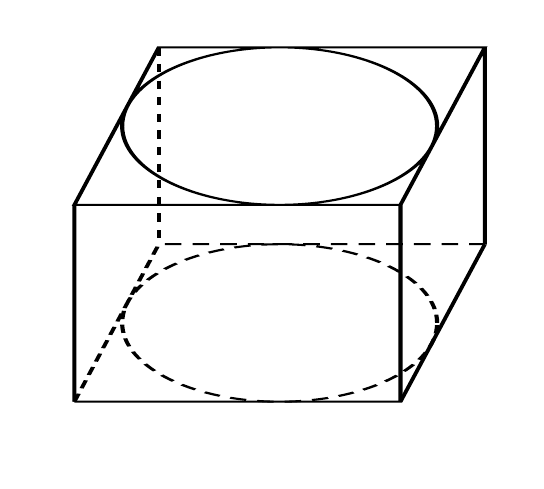
\begin{tikzpicture}
				\clip (-3.2,-1.75) rectangle (3,3.75);
				\draw[transform canvas={cm={2,0,0,1,(0,0)}},densely dashed]
				(-1,-1) coordinate (At)  (1,-1) coordinate (Bt) 
				(-1,1) coordinate (Ct) (1,1) coordinate (Dt) 
				(0,0) circle (1)
				(-15:1) coordinate (Tm)
				([rotate around={90:(Tm)}]0,0) coordinate (Ap)
				(intersection of Ap--Tm and At--Bt) coordinate (B)
				(intersection of Ap--Tm and Ct--Dt) coordinate (C)
				(165:1) coordinate (Th)
				([rotate around={90:(Th)}]0,0) coordinate (Ap)
				(intersection of Ap--Th and At--Bt) coordinate (A)
				(intersection of Ap--Th and Ct--Dt) coordinate (D)
				(A)--(D)--(C);
				\draw[transform canvas={cm={2,0,0,1,(0,0)}}] 
				(A)--(B)--(C);
				\draw[transform canvas={cm={2,0,0,1,(0,2.5)}}]
				(-1,-1) coordinate (At)  (1,-1) coordinate (Bt) 
				(-1,1) coordinate (Ct) (1,1) coordinate (Dt) 
				(0,0) circle (1)
				(-15:1) coordinate (Tm)
				([rotate around={90:(Tm)}]0,0) coordinate (Ap)
				(intersection of Ap--Tm and At--Bt) coordinate (B')
				(intersection of Ap--Tm and Ct--Dt) coordinate (C')
				(165:1) coordinate (Th)
				([rotate around={90:(Th)}]0,0) coordinate (Ap)
				(intersection of Ap--Th and At--Bt) coordinate (A')
				(intersection of Ap--Th and Ct--Dt) coordinate (D')
				(C')--(B')--(A')--(D')--cycle
				\foreach \x in {B',A',C'}{
					(\x)--+(0,-2.5)};
				\draw[transform canvas={cm={2,0,0,1,(0,2.5)}},dashed]
				(D')--+(0,-2.5);
			\end{tikzpicture}
		\end{center}
		Ta có: $S_1=6.40^2=9600$.\\
		Bán kính đường tròn nội tiếp hai mặt đối diện của hình lập phương là: $ r=20\text{cm}$; hình trụ có đường sinh $ h=40\text{cm}$\\
		Diện tích toàn phần của hình trụ là: $S_2=2.\pi{20^2}+2\pi .20.40=2400\pi $.\\
		Vậy: $ S=S_1+S_2=9600+2400\pi=2400\left(4+\pi\right)$.}
\end{ex}

\begin{ex}%Câu 13 [2H2B1-2]
%	[Chuyên Quốc Học Huế 2018] 
	Một hình trụ có diện tích xung quanh bằng $ 4\pi $, thiết diện qua trục là hình vuông. Một mặt phẳng $\left(\alpha\right)$ song song với trục, cắt hình trụ theo thiết diện là tứ giác $ AB{B}'{A}'$, biết một cạnh của thiết diện là một dây cung của đường tròn đáy của hình trụ và căng một cung $ 120^\circ $. Tính diện tích thiết diện $ AB{B}'{A}'$.
	\choice
	{$ 3\sqrt{2}$}
	{$\sqrt{3}$}
	{\True $ 2\sqrt{3}$}
	{$ 2\sqrt{2}$}
	\loigiai{
	\begin{center}
	\begin{tikzpicture}
		\draw (0,0) ellipse (2cm and 0.6cm);
		\draw (-2,0) -- (-2,-4);
		\draw (2,0) -- (2,-4);
		\draw (-2,-4) arc (180:360:2cm and 0.6cm);
		\draw[dashed] (2,-4) arc (0:180:2cm and 0.6cm);
		\fill (0,0) circle (1.5pt);
		\fill (0,-4) circle (1.5pt);
		\node[draw,fill,circle,inner sep=1pt,label={-80:$A$}] (D) at (-75:2cm and 0.6cm) {};
		\node[draw,fill,circle,inner sep=1pt,label={90:$B$}] (C) at (35:2cm and 0.6cm) {};
		\node[draw,fill,circle,inner sep=1pt,label={-90:$A'$}] (A) at ($(0,-4)+(-75:2 and 0.6)$) {};
		\node[draw,fill,circle,inner sep=1pt,label={110:$B'$}] (B) at ($(0,-4)+(35:2 and 0.6)$) {};
		\draw (-75:2cm and 0.6cm) -- ($(0,-4)+(-75:2 and 0.6)$);
		\draw[dashed] (35:2cm and 0.6cm) -- ($(0,-4)+(35:2 and 0.6)$);
		\node[left] at (0,0) {$O$};
		\node[left] at (0,-4) {$O'$};
		%		\coordinate (H) at ($(A)!0.5!(B)$);
		\draw[dashed] (A) -- (0,-4) -- (B)--(A) (0,0)--(0,-4);
		\draw (D) -- (0,0) -- (C)--(D);
		%		\fill (H) circle (1.5pt);
		%		\node[right] at (H) {$H$};
	\end{tikzpicture}
\end{center}
		Gọi $ R$, $ h$, $ l$ lần lượt là bán kính, chiều cao, đường sinh của hình trụ.\\
		Ta có $S_{xq}=4\pi $$\Leftrightarrow 2\pi .R.l=4\pi $$\Leftrightarrow R.l=2$.\\
		Giả sử $ AB$ là một dây cung của đường tròn đáy của hình trụ và căng một cung $ 120^\circ $.\\
		Ta có $ AB{B}'{A}'$ là hình chữ nhật có $ A{A}'=h=l$.\\
		Xét tam giác $ OAB$ cân tại $ O$, $ OA=OB=R$, $\widehat{AOB}=120^\circ $$\Rightarrow AB=R\sqrt{3}$.\\
		$S_{AB{B}'{A}'}=AB.A{A}'$$=R\sqrt{3}.l$$=R.l\sqrt{3}$$=2\sqrt{3}$.}
\end{ex}

\begin{ex}%Câu 14 [2H2B1-2]
%	[Chuyên Lương Thế Vinh-Đồng Nai-2018] 
	Ba chiếc bình hình trụ cùng chứa $ 1$ lượng nước như nhau, độ cao mực nước trong bình $ II$ gấp đôi bình $ I$ và trong bình $ III$ gấp đôi bình $ II$. Chọn nhận xét đúng về bán kính đáy $r_1$, $r_2$, $r_3$ của ba bình $I$, $II$, $ III$.
	\choice
	{$r_1$, $r_2$, $r_3$ theo thứ tự lập thành cấp số nhân công bội $ 2$}
	{$r_1$, $r_2$, $r_3$ theo thứ tự lập thành cấp số nhân công bội $\dfrac{1}{2}$}
	{$r_1$, $r_2$, $r_3$ theo thứ tự lập thành cấp số nhân công bội $\sqrt{2}$}
	{\True $r_1$, $r_2$, $r_3$ theo thứ tự lập thành cấp số nhân công bội $\dfrac{1}{\sqrt{2}}$}
	\loigiai{
		Gọi $V_1$, $V_2$, $V_3$ lần lượt là thể tích của bình $I$, $ II$, $III$.\\
		Ta có\\
		$~{V_1}=V_2$ $\Leftrightarrow\pi{r_1}^2h_1=\pi{r_2}^2h_2$ $\Leftrightarrow{r_1}^2h_1=r_2^22h_1$ $\Rightarrow{r_2}=\dfrac{r_1}{\sqrt{2}}\,\,(1)$ .\\
		$~{V_2}=V_3$ $\Leftrightarrow\pi{r_2}^2h_2=\pi{r_3}^2h_3$ $\Leftrightarrow{r_2}^2h_2=r_3^22h_2$ $\Rightarrow{r_3}=\dfrac{r_2}{\sqrt{2}}\,\,(2)$ .\\
		Từ $(1)$ và $(2)$ ta có $r_1$, $r_2$, $r_3$ theo thứ tự lập thành cấp số nhân công bội $\dfrac{1}{\sqrt{2}}$.}
\end{ex}

\begin{ex}%Câu 15 [2H2B1-2]
%	[Chuyên Thái Bình-2018] 
	Cho hình trụ có bán kính đáy bằng $ R$ và chiều cao bằng $\dfrac{3R}{2}$. Mặt phẳng $\left(\alpha\right)$ song song với trục của hình trụ và cách trục một khoảng bằng $\dfrac{R}{2}$. Tính diện tích thiết diện của hình trụ cắt bởi mặt phẳng $\left(\alpha\right)$.
	\choice
	{$\dfrac{2R^2\sqrt{3}}{3}$}
	{\True $\dfrac{3R^2\sqrt{3}}{2}$}
	{$\dfrac{3R^2\sqrt{2}}{2}$}
	{$\dfrac{2R^2\sqrt{2}}{3}$}
	\loigiai{
		\begin{center}
\begin{tikzpicture}
	\coordinate[label=below left:$O$] (O)at(0,0);
	\fill[black] (O)circle(0.2pt);
	\draw[black] (O) circle (2cm);
	\coordinate[label=above left:$A$] (A) at ($(O)+(120:2)$);
	\coordinate[label=right:$B$] (B) at ($(O)+(0:2)$);\draw[black] (A)--(B);
	\draw[black] (A)--(O);
	\draw[black] (B)--(O);
	\path (A)--(B)node[pos=0.5,sloped,black,above right]{$m$};
\end{tikzpicture}
		\end{center}
		Thiết diện của hình trụ cắt bởi mặt phẳng $\left(\alpha\right)$ là hình chữ nhật $ ABCD$ với $ BC=\dfrac{3R}{2}$.\\
		Gọi $ H$ là trung điểm $ AB$, ta có $ AH=\dfrac{R}{2}$$\Rightarrow AB=2HB=2\sqrt{R^2-A{H^2}}=R\sqrt{3}$.\\
		Vậy diện tích thiết diện là: $ S=AB.CD=R\sqrt{3}.\dfrac{3R}{2}=\dfrac{3R^2\sqrt{3}}{2}$.}
\end{ex}

\begin{ex}%Câu 16 [2H2B1-2]
%	[THPT Hải An-Hải Phòng-2018] 
	Cho hình trụ có bán kính đáy bằng $5\,\text{cm}$ và khoảng cách giữa hai đáy là $7\,\text{cm}$ . Cắt khối trụ bởi một mặt phẳng song song với trục và cách trục $3\,\text{cm}$ . Tính diện tích $S$ của thiết diện được tạo thành.
	\choice
	{$55\,\text{c}{\text{m}^{\text{2}}}$}
	{\True $56\,\text{c}{\text{m}^{\text{2}}}$}
	{$53\,\text{c}{\text{m}^{\text{2}}}$}
	{$46\,\text{c}{\text{m}^{\text{2}}}$}
	\loigiai{
\begin{center}
\begin{tikzpicture}
	\draw (0,0) ellipse (2cm and 0.6cm);
	\draw (-2,0) -- (-2,-4);
	\draw (2,0) -- (2,-4);
	\draw (-2,-4) arc (180:360:2cm and 0.6cm);
	\draw[dashed] (2,-4) arc (0:180:2cm and 0.6cm);
	\fill (0,0) circle (1.5pt);
	\fill (0,-4) circle (1.5pt);
	\node[draw,fill,circle,inner sep=1pt,label={-80:$D$}] (D) at (-75:2cm and 0.6cm) {};
	\node[draw,fill,circle,inner sep=1pt,label={90:$C$}] (C) at (35:2cm and 0.6cm) {};
	\node[draw,fill,circle,inner sep=1pt,label={-90:$A$}] (A) at ($(0,-4)+(-75:2 and 0.6)$) {};
	\node[draw,fill,circle,inner sep=1pt,label={-90:$B$}] (B) at ($(0,-4)+(35:2 and 0.6)$) {};
	\draw (-75:2cm and 0.6cm) -- ($(0,-4)+(-75:2 and 0.6)$);
	\draw[dashed] (35:2cm and 0.6cm) -- ($(0,-4)+(35:2 and 0.6)$);
	\node[left] at (0,0) {$O$};
	\node[left] at (0,-4) {$O'$};
	\coordinate (H) at ($(D)!0.5!(C)$);
	\draw[dashed] (A) -- (0,-4) -- (B)--(A) (0,0)--(0,-4);
	\draw (D) -- (0,0) -- (C)--(D) (0,0)--(H);
	\fill (H) circle (1.5pt);
	\node[right] at (H) {$H$};
\end{tikzpicture}
\end{center}
		Gọi thiết diện là hình chữ nhật $ABCD$ , $H$ là trung điểm $CD$ .\\
		Ta có: $\left\{\begin{aligned}
			& OH\perp CD\\ 
			& OH\perp BC\\ 
		\end{aligned}\right.\Rightarrow OH\perp (ABCD)$ $\Rightarrow d\left(O{O}';(ABCD)\right)=d\left(O;(ABCD)\right)=OH=3\,cm$ .\\
		$\Rightarrow HC=HD=\sqrt{OC^2-OH^2}=\sqrt{5^2-3^2}=4\,\text{cm}$ .\\
		$\Rightarrow AB=CD=8\,\text{cm}$ .\\
		$\Rightarrow{S_{ABCD}}=AB.BC=8.7=56\,\text{c}{\text{m}^{\text{2}}}$ .}
\end{ex}

\begin{ex}%Câu 17 [2H2B1-2]
%	[Chuyên Hạ Long-2018] 
	Cho hình trụ có chiều cao bằng $6\sqrt{2}\,cm$ . Biết rằng một mặt phẳng không vuông góc với đáy và cắt hai mặt đáy theo hai dây cung song song $AB$ , $A'{B}'$ mà $AB=A'{B}'=6\,cm$ , diện tích tứ giác $AB{B}'{A}'$ bằng $60\,c{m^2}$ . Tính bán kính đáy của hình trụ.
	\choice
	{$5\,cm$}
	{$3\sqrt{2}\,cm$}
	{\True $4\,cm$}
	{$5\sqrt{2}\,cm$}
	\loigiai{
		\begin{center}
			\begin{tikzpicture}[>=stealth,line join=round,line cap=round,font=\footnotesize,scale=1,declare function={a=2;b=a/2;h=4;}]
				\path
				(0,0)coordinate(O')
				(0,h)	coordinate(O)
				(115:a and a/2)coordinate(A1)
				(220:a and a/2)coordinate(B1)
				($(A1)+(90:h)$)coordinate(A)
				($(B1)+(90:h)$)coordinate(B)
				($(O')-(A1)$)coordinate (B') 
				($(O')-(B1)$)coordinate (A') 
				($(A')!1/2!(B')$)coordinate (M')
				($(A)!1/2!(B)$)coordinate (M)
				;
				\draw (a,h)--(a,0)arc (0:-180:a and b)--(-a,h);
				\draw[dashed] (a,0)arc (0:180:a and b);
				\draw (O)ellipse (a and b);
				\draw (B1)--(B)--(B') (A)--(B);
				\draw[dashed] (A1)--(A)--(A')
				(B1)--(A1)--(A')--(B')--(B1)
				(O)--(O')--(M')--(M)
				;
				\fill (-a,h/2)node[left]{$6\sqrt{2}$}
				(M)+(-180:.25)node{$6$}
				(A1)circle(1pt)+(150:.25)node{$A_1$}
				(B1)circle(1pt)+(-150:.25)node{$B_1$}
				;
				\foreach \i \g in {A/90,B/-150,O/50,O'/180,A'/50,B'/-90}\fill(\i)circle(1pt)+(\g:.25)node{$\i$};
				\draw pic[draw,angle radius=5pt]{right angle=A1--B1--B'};
				\draw pic[draw,angle radius=5pt]{right angle=O'--M'--B'};
			\end{tikzpicture}
		\end{center}
		Gọi $O$, $O'$ là tâm các đáy hình trụ (hình vẽ).\\
		Vì $AB=A'{B}'$ nên $\left(AB{B}'{A}'\right)$ đi qua trung điểm của đoạn $O{O}'$ và $ AB{B}'{A}'$ là hình chữ nhật.\\
		Ta có $S_{AB{B}'{A}'}=AB.A{A}'$ $\Leftrightarrow 60=6.A{A}'$ $\Rightarrow A{A}'=10\left(cm\right)$.\\
		Gọi $A_1$, $B_1$ lần lượt là hình chiếu của $ A$, $ B$ trên mặt đáy chứa $A'$ và $B'$\\
		$\Rightarrow{A}'{B}'{B_1}{A_1}$ là hình chữ nhật có $A'{B}'=6\left(cm\right)$,\\
		$B_1B'=\sqrt{B{B'^2}-B{B_1}^2}$ $=\sqrt{10^2-\left(6\sqrt{2}\right)^2}$ $=2\sqrt{7}\left(cm\right)$\\
		Gọi $R$ là bán kính đáy của hình trụ, ta có 		$2R=A'{B_1}=\sqrt{B_1B'^2+A'{B'^2}}=8$ $\Rightarrow R=4\left(cm\right)$.}
\end{ex}

\begin{ex}%Câu 18 [2H2B1-2]
%	[Chuyên Thái Bình-2018]
	 Một hình trụ có bán kính đáy $ r=5\,\text{cm}$ và khoảng cách giữa hai đáy $ h=7\,\text{cm}$. Cắt khối trụ bởi một mặt phẳng song song với trục và cách trục $ 3\,\text{cm}$. Diện tích của thiết diện được tạo thành là:
	\choice
	{\True $ S=56\left(\text{c}{\text{m}^{\text{2}}}\right)$}
	{$ S=55\left(\text{c}{\text{m}^{\text{2}}}\right)$}
	{$ S=53\left(\text{c}{\text{m}^{\text{2}}}\right)$}
	{$ S=46\left(\text{c}{\text{m}^{\text{2}}}\right)$}
	\loigiai{
		Gọi $ O,O'$ là tâm của hai đáy của hình trụ và $(P)$ là mặt phẳng song song với trục và cách trục $ O{O}'$ một khoảng $ 3\text{cm}$.\\
		Mp$(P)$ cắt hai hình tròn đáy $(O),\left(O'\right)$ theo hai dây cung lần lượt là $ AB,\,CD$ và cắt mặt xung quanh theo hai đường sinh là $AD,BC$ . Khi đó $ABCD$ là hình chữ nhật.\\
	\begin{center}
		\begin{tikzpicture}
			\draw (0,0) ellipse (2cm and 0.6cm);
			\draw (-2,0) -- (-2,-4);
			\draw (2,0) -- (2,-4);
			\draw (-2,-4) arc (180:360:2cm and 0.6cm);
			\draw[dashed] (2,-4) arc (0:180:2cm and 0.6cm);
			\fill (0,0) circle (1.5pt);
			\fill (0,-4) circle (1.5pt);
			\node[draw,fill,circle,inner sep=1pt,label={-80:$D$}] (D) at (-75:2cm and 0.6cm) {};
			\node[draw,fill,circle,inner sep=1pt,label={90:$C$}] (C) at (35:2cm and 0.6cm) {};
			\node[draw,fill,circle,inner sep=1pt,label={-90:$A$}] (A) at ($(0,-4)+(-75:2 and 0.6)$) {};
			\node[draw,fill,circle,inner sep=1pt,label={110:$B$}] (B) at ($(0,-4)+(35:2 and 0.6)$) {};
			\draw (-75:2cm and 0.6cm) -- ($(0,-4)+(-75:2 and 0.6)$);
			\draw[dashed] (35:2cm and 0.6cm) -- ($(0,-4)+(35:2 and 0.6)$);
			\node[left] at (0,0) {$O'$};
			\node[left] at (0,-4) {$O$};
			\coordinate (H) at ($(A)!0.5!(B)$);
			\draw[dashed] (A) -- (0,-4) -- (B)--(A) (0,0)--(0,-4)--(H);
			\draw (D) -- (0,0) -- (C)--(D);
			\fill (H) circle (1.5pt);
			\node[right] at (H) {$H$};
		\end{tikzpicture}
	\end{center}
		Gọi $H$ là trung điểm của $ AB$. Ta có $ OH\perp AB;OH\perp AD\Rightarrow OH\perp\left(ABCD\right)$\\
		$\Rightarrow d\left(O\,O',(P)\right)=d\left(O,\left(ABCD\right)\right)=OH=3\text{cm}$.\\
		Khi đó: $ AB=2AH=2\sqrt{O{A^2}-O{H^2}}=2\sqrt{5^2-3^2}=8$; $ AD=O\,O'=h=7\text{cm}$.\\
		Diện tích hình chữ nhật $ ABCD$ là: $S_{ABCD}=AB.AD=56\left(c{m^2}\right)$.}
\end{ex}
%%%---19-27-----
	\begin{ex}%Câu 19 [2H2B1-2]
%	(Chuyên Thái Bình-2018) 
	Cho hình trụ có hai đáy là hai hình tròn $(O)$ và $\left(O'\right)$, chiều cao $ 2R$ và bán kính đáy $ R$. Một mặt phẳng $\left(\alpha\right)$ đi qua trung điểm của $ O{O}'$ và tạo với $ O{O}'$ một góc $ 30^\circ $. Hỏi $\left(\alpha\right)$ cắt đường tròn đáy theo một dây cung có độ dài bằng bao nhiêu?
	\choice
	{\True $\dfrac{2R\sqrt{2}}{\sqrt{3}}$}
	{$\dfrac{4R}{3\sqrt{3}}$}
	{$\dfrac{2R}{3}$}
	{$\dfrac{2R}{\sqrt{3}}$}
	\loigiai{
		\begin{center}
			\begin{tikzpicture}
				\draw (0,0) ellipse (2cm and 0.6cm);
				\draw (-2,0) -- (-2,-4);
				\draw (2,0) -- (2,-4);
				\draw (-2,-4) arc (180:360:2cm and 0.6cm);
				\draw[dashed] (2,-4) arc (0:180:2cm and 0.6cm);
				\fill (0,0) circle (1.5pt);
				\fill (0,-4) circle (1.5pt);
				\node[draw,fill,circle,inner sep=1pt,label={-90:$B$}] (B) at (-30:2cm and 0.6cm) {};
				\node[draw,fill,circle,inner sep=1pt,label={90:$A$}] (A) at (60:2cm and 0.6cm) {};
				\node[above] (O) at (0,0) {O};
				\node[below] (O') at (0,-4) {O'};
				\coordinate (M) at ($(O)!0.5!(O')$);
				\coordinate (D) at ($(B)!2!(M)$);
				\coordinate (C) at ($(A)!2!(M)$);
				\coordinate (H) at ($(A)!0.5!(B)$);
				\coordinate (K) at ($(H)!0.4!(M)$);
				\node[draw,fill,circle,inner sep=1pt,label={90:$M$}] at (M) {};
				\node[draw,fill,circle,inner sep=1pt,label={90:$C$}] at (C) {};
				\node[draw,fill,circle,inner sep=1pt,label={90:$D$}] at (D) {};
				\node[draw,fill,circle,inner sep=1pt,label={0:$H$}] at (H) {};
				\node[draw,fill,circle,inner sep=1pt,label={-90:$K$}] at (K) {};
				\draw (A) -- (0,0) -- (B) -- (A);
				\draw[dashed] (B) -- (C) -- (D)-- (A);
				\draw[dashed] (M)--(H)--(0,0) -- (0,-4);
				\draw[dashed] (0,0) -- (K);
			\end{tikzpicture}
		\end{center}
		Gọi $ M$ là trung điểm của $ O{O}'$. Gọi $ A$, $ B$ là giao điểm của mặt phẳng $\left(\alpha\right)$ và đường tròn $(O)$ và $ H$ là hình chiếu của $ O$ trên $ AB$ $\Rightarrow AB\perp\left(MHO\right)$.\\
		Trong mặt phẳng $\left(MHO\right)$ kẻ $ OK\perp MH$, $\left(K\in MH\right)$ khi đó góc giữa $ O{O}'$ và mặt phẳng $\left(\alpha\right)$ là góc $\widehat{OMK}=30^\circ $.\\
		Xét tam giác vuông $ MHO$ ta có $ HO=OM\tan 30^\circ $$=R\tan 30^\circ $$=\dfrac{R\sqrt{3}}{3}$.\\
		Xét tam giác vuông $ AHO$ ta có $ AH=\sqrt{O{A^2}-O{H^2}}$$=\sqrt{R^2-\dfrac{R^2}{3}}$$=\dfrac{R\sqrt{2}}{\sqrt{3}}$.\\
		Do $ H$ là trung điểm của $ AB$ nên $ AB=\dfrac{2R\sqrt{2}}{\sqrt{3}}$.}
\end{ex}

\begin{ex}%Câu 20 [2H2B1-2]
%	(THPT Lê Xoay-2018)
	 Một cốc nước hình trụ có chiều cao $\text{9cm}$, đường kính $\text{6cm}$. Mặt đáy phẳng dày $\text{1cm}$, thành cốc dày $\text{0}\text{,2}\,\text{cm}$. Đổ vào cốc $\text{120 ml}$ nước sau đó thả vào cốc $\text{5}$ viên bi có đường kính $\text{2cm}$. Mặt nước cách mép cốc gần nhất với giá trị bằng
	\choice
	{$\text{3}\text{,67}\left(\text{cm}\right)$}
	{$\text{3}\text{,08}\left(\text{cm}\right)$}
	{\True $ 2,28\left(\text{cm}\right)$}
	{$ 2,62\left(\text{cm}\right)$}
	\loigiai{
		Thể tích của cốc nước là: $V=\pi \cdot\left(2,8\right)^2\cdot 8$ $=62,72\pi\left(\text{c}{\text{m}^{\text{3}}}\right)$ .\\
		Thể tích của $\text{5}$ viên bi là: $V_1=5\cdot \dfrac{4}{3}\cdot \pi{1^3}$ $=\dfrac{20}{3}\cdot \pi\left(\text{c}{\text{m}^{\text{3}}}\right)$ .\\
		Thể tích còn lại sau khi đổ vào cốc $\text{120 ml}$ nước và thả vào cốc $\text{5}$ viên bi là: $V_2=V-V_1-120$ $=62,72\pi-\dfrac{20}{3}\cdot \pi-120$ $\approx 56,10\left(\text{c}{\text{m}^{\text{3}}}\right)$ .\\
		Chiều cao phần còn lại là: $h=\dfrac{V_2}{\pi \cdot (2,8)^2}$ $\approx\dfrac{56,10}{\pi \cdot (2,8)^2}$ $\approx 2,28\left(\text{cm}\right)$ .}
\end{ex}

\begin{ex}%Câu 21 [2H2B1-2]
%	(Chuyên Nguyễn Bỉnh Khiêm-Quảng Nam-2020)
	 Cho hình trụ có bán kính đáy bằng $ R$ và chiều cao bằng $\dfrac{3R}{2}$. Mặt phẳng $\left(\alpha\right)$ song song với trục của hình trụ và cách trục một khoảng bằng $\dfrac{R}{2}$. Diện tích thiết diện của hình trụ cắt bởi mặt phẳng $\left(\alpha\right)$ là:
	\choice
	{$\dfrac{3\sqrt{2}{R^2}}{2}$}
	{\True $\dfrac{3\sqrt{3}{R^2}}{2}$}
	{$\dfrac{2\sqrt{3}{R^2}}{3}$}
	{$\dfrac{2\sqrt{2}{R^2}}{3}$}
	\loigiai{
	\begin{center}
	\begin{tikzpicture}
		\draw (0,0) ellipse (2cm and 0.6cm);
		\draw (-2,0) -- (-2,-4);
		\draw (2,0) -- (2,-4);
		\draw (-2,-4) arc (180:360:2cm and 0.6cm);
		\draw[dashed] (2,-4) arc (0:180:2cm and 0.6cm);
		\fill (0,0) circle (1.5pt);
		\fill (0,-4) circle (1.5pt);
		\node[draw,fill,circle,inner sep=1pt,label={-80:$D$}] (D) at (-75:2cm and 0.6cm) {};
		\node[draw,fill,circle,inner sep=1pt,label={90:$C$}] (C) at (35:2cm and 0.6cm) {};
		\node[draw,fill,circle,inner sep=1pt,label={-90:$A$}] (A) at ($(0,-4)+(-75:2 and 0.6)$) {};
		\node[draw,fill,circle,inner sep=1pt,label={110:$B$}] (B) at ($(0,-4)+(35:2 and 0.6)$) {};
		\draw (-75:2cm and 0.6cm) -- ($(0,-4)+(-75:2 and 0.6)$);
		\draw[dashed] (35:2cm and 0.6cm) -- ($(0,-4)+(35:2 and 0.6)$);
		\node[left] at (0,0) {$O'$};
		\node[left] at (0,-4) {$O$};
		\coordinate (H) at ($(A)!0.5!(B)$);
		\draw[dashed] (A) -- (0,-4) -- (B)--(A) (0,0)--(0,-4)--(H);
		\draw (D) -- (0,0) -- (C)--(D);
		\fill (H) circle (1.5pt);
		\node[right] at (H) {$H$};
	\end{tikzpicture}
\end{center}
		Giả sử thiết diện là hình chữ nhật $ ABCD$ như hình vẽ.\\
		Gọi H là trung điểm của $ AB$ suy ra $ OH\perp AB$ suy ra $ \mathrm{d}\left(O;AB\right)=\dfrac{R}{2}$.\\
		Khi đó $AB=2HA=2\sqrt{OA^2-OH^2}=2\sqrt{R^2-\left(\dfrac{R}{2}\right)^2}=R\sqrt{3}$.\\
		Suy ra $S_{ABCD}=AB.BC=R\sqrt{3}.\dfrac{3R}{2}=\dfrac{3\sqrt{3}{R^2}}{2}$ .}
\end{ex}

%%%---Bỏ câu 22 trùng câu 13
\begin{ex}%Câu 23 [2H2B1-2]
%	(Liên trường Nghệ An-2020) 
	Một sợi dây (không co giản) được quấn đối xứng đúng $10$ vòng quanh một ống trụ tròn đều có bán kính $R=\dfrac{2}{\pi}$ cm (Như hình vẽ)
	\begin{center}
		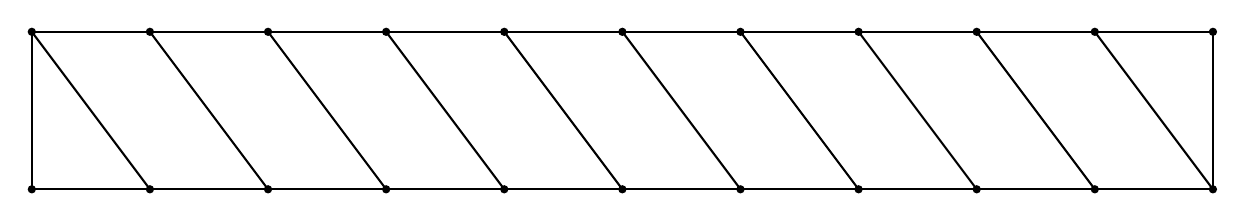
\begin{tikzpicture}
			\draw (0,0) rectangle (15,2);
			\foreach \x in {0,1,2,3,4,5,6,7,8,9,10}
			\fill (1.5*\x,0) circle (1.5pt);
			\foreach \x in {0,1,2,3,4,5,6,7,8,9,10}
			\fill (1.5*\x,2) circle (1.5pt);
			\foreach \x in {0,1,2,3,4,5,6,7,8,9}
			\draw (1.5*\x,2) -- (1.5*\x+1.5,0);
		\end{tikzpicture}
	\end{center}
	Biết rằng sợi dây dài $50$ cm. Hãy tính diện tích xung quanh của ống trụ đó.
	\choice
	{$80$ cm$^2$}
	{$100$ cm$^2$}
	{$60$ cm$^2$}
	{\True $120$ cm$^2$}
	\loigiai{
		Khi trải phẳng ống trụ tròn đều ta được một hình chữ nhật có chiều rộng là chu vi của mặt đáy còn chiều dài là chiều dài của trụ, mỗi vòng quấn của dây dài $ 5$ cm là đường chéo của hình chữ nhật có kích thước lần lượt bằng chu vi đáy trụ và $\dfrac{1}{10}$ chiều dài trụ (hình vẽ).
		\begin{center}
			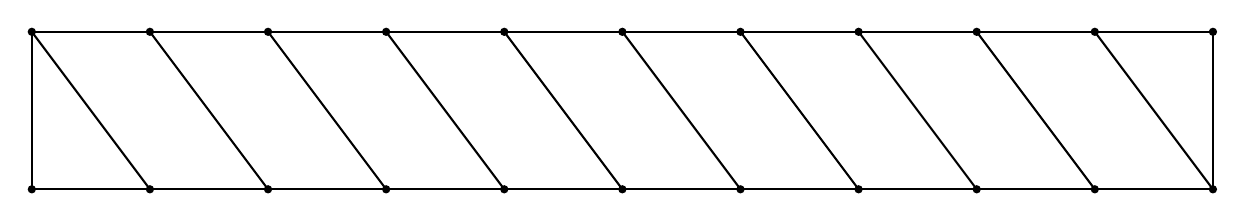
\begin{tikzpicture}
				\draw (0,0) rectangle (15,2);
				\foreach \x in {0,1,2,3,4,5,6,7,8,9,10}
				\fill (1.5*\x,0) circle (1.5pt);
				\foreach \x in {0,1,2,3,4,5,6,7,8,9,10}
				\fill (1.5*\x,2) circle (1.5pt);
				\foreach \x in {0,1,2,3,4,5,6,7,8,9}
				\draw (1.5*\x,2) -- (1.5*\x+1.5,0);
			\end{tikzpicture}
		\end{center}
		Gọi chiều dài trụ là $ l\left(cm\right)$,theo định lí Pytago ta có $\sqrt{5^2-\left(2\cdot \dfrac{2}{\pi}\pi\right)^2}=\dfrac{l}{10}\Leftrightarrow l=30$(cm).\\
		Vậy diện tích xung quanh của trụ là: $S_{xq}=2\cdot \dfrac{2}{\pi}\cdot \pi \cdot 30=120$ (cm$^2$).}
\end{ex}

\begin{ex}%Câu 24 [2H2B1-2]
%	(THPT Nguyễn Viết Xuân-2020)
	 Một cái mũ bằng vải của nhà ảo thuật với kích thước như hình vẽ. Hãy tính tổng diện tích vải cần có để làm nên cái mũ đó (không tính viền, mép, phần thừa).
	\begin{center}
		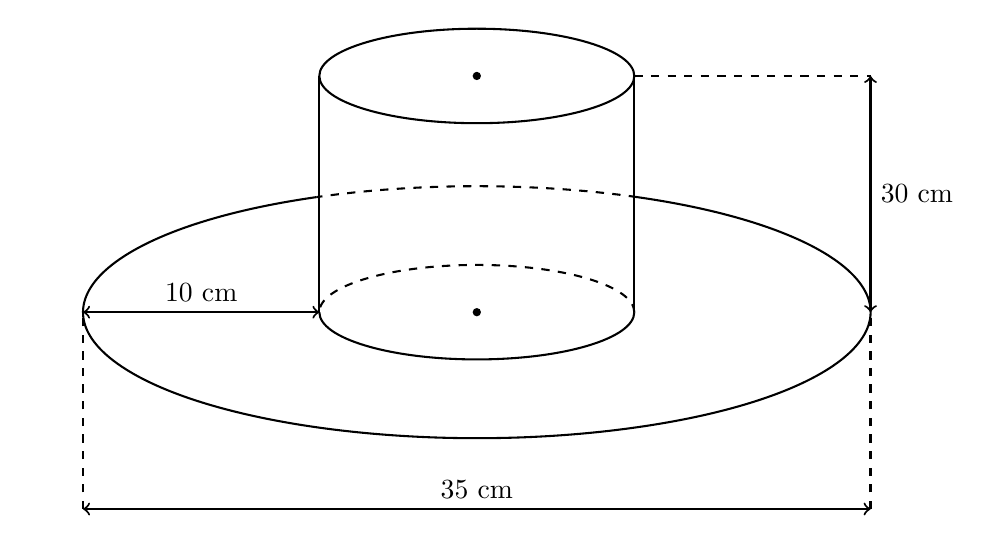
\begin{tikzpicture}
			\draw (0,0) ellipse (2cm and 0.6cm);
			\draw (-2,0) -- (-2,-3);
			\draw (2,0) -- (2,-3);
			\draw (-2,-3) arc (180:360:2cm and 0.6cm);
			\draw[dashed] (2,-3) arc (0:180:2cm and 0.6cm);
			\fill (0,0) circle (1.5pt);
			\fill (0,-3) circle (1.5pt);
			\draw (0,-3)+(114: 5 and 1.6) arc (114:426:5cm and 1.6cm);
			\draw[dashed] (0,-3)+(66: 5 and 1.6) arc (66:114:5 and 1.6);
			\draw [<->] (-5,-3)node{} -- (-3.5,-3)node[above]{$10$ cm} -- (-2,-3)node{};
			\draw [<->] (-5,-5.5)node{} -- (0,-5.5)node[above]{$35$ cm} -- (5,-5.5)node{};
			\draw [<->] (5,0)node{} -- (5,-1.5)node[right]{$30$ cm} -- (5,-3)node{};
			\draw[dashed] (-5,-5.5) -- (-5,-3);
			\draw[dashed] (5,-5.5) -- (5,-3);
			\draw[dashed] (2,0) -- (5,0);
		\end{tikzpicture}
	\end{center}
	\choice
	{$ 750,25\pi$ cm$^2$}
	{\True $ 756,25\pi$ cm$^2$}
	{$ 700\pi$ cm$^2$}
	{$ 700\pi$ cm$^2$}
	\loigiai{
		Bán kính hình trụ của cái mũ là $ r=\dfrac{35-10-10}{2}=\dfrac{15}{2}$ (cm).\\
		Đường cao hình trụ của cái mũ là $ 30$ cm.\\
		Diện tích xung hình trụ là: $S_{xq}=2\pi r\ell=2\cdot\pi \cdot\dfrac{15}{2}\cdot30=450\pi$ (cm$^2$).\\
		Diện tích vành mũ là: $S_v=\pi{\left(\dfrac{35}{2}\right)^2}-S_d$ (cm$^2$).\\
		Vậy tổng diện tích vải cần có để làm nên cái mũ đó (không tính viền, mép, phần thừa) là:\\
		$ S=S_{xq}+S_d+S_v=450\pi+\left(\dfrac{35}{2}\right)^2\pi=756,25\cdot\pi$ (cm$^2$).
	}
\end{ex}

\begin{ex}%Câu 25 [2H2B1-2]
%	(Hải Hậu-Nam Định-2020) 
	Một khối trụ có bán kính đáy $r=2a$. $O,\,O'$ lần lượt là tâm đường tròn đáy. Một mặt phẳng song song với trục và cách trục $\dfrac{a\sqrt{15}}{2}$ , cắt đường tròn $\left(O'\right)$ tại hai điểm $A$, $B$. Biết thể tích của khối tứ diện $O{O}'AB$ bằng $\dfrac{a^3\sqrt{15}}{4}$ . Độ dài đường cao của hình trụ bằng
	\choice
	{$ a$}
	{$ 6a$}
	{\True $ 3a$}
	{$ 2a$}
	\loigiai{
		\begin{center}
			\begin{tikzpicture}
				\draw (0,0) ellipse (2cm and 0.6cm);
				\draw (-2,0) -- (-2,-4);
				\draw (2,0) -- (2,-4);
				\draw (-2,-4) arc (180:360:2cm and 0.6cm);
				\draw[dashed] (2,-4) arc (0:180:2cm and 0.6cm);
				\fill (0,0) circle (1.5pt);
				\fill (0,-4) circle (1.5pt);
				\node[draw,fill,circle,inner sep=1pt,label={90:$C$}] (C) at (-70:2cm and 0.6cm) {};
				\node[draw,fill,circle,inner sep=1pt,label={-90:$A$}] (A) at ($(0,-4)+(-70:2 and 0.6)$) {};
				\node[draw,fill,circle,inner sep=1pt,label={30:$B$}] (B) at ($(0,-4)+(45:2 and 0.6)$) {};
				\draw (-70:2cm and 0.6cm) -- ($(0,-4)+(-70:2 and 0.6)$);
				\node[above] at (0,0) {O};
				\node[below] at (0,-4) {O'};
				\coordinate (I) at ($(A)!0.5!(B)$);
				\draw[dashed] (A) -- (0,-4) -- (B)--(A) (I)--(0,-4)--(0,0) (A)--(0,0)--(B) (C)--(B);
				\fill (I) circle (1.5pt);
				\node[right] at (I) {I};
			\end{tikzpicture}
		\end{center}
		Vẽ đường sinh $AC$, khi đó mặt phẳng $\left(ABC\right)$ song song với $O{O}'$ và cách $O{O}'$ một khoảng $\dfrac{a\sqrt{15}}{2}$ .\\
		Gọi $I$ là trung điểm $AB$ , ta có $d\left(O{O}',\left(ABC\right)\right)=\mathrm{d}\left(O',\left(ABC\right)\right)=O'I=\dfrac{a\sqrt{15}}{2}$.\\
		Bán kính $O'A=2a$ suy ra $BA=2IA=2\sqrt{O'{A^2}-O'{I^2}}=2\sqrt{4a^2-\dfrac{15a^2}{4}}=a$ .\\
		Thể tích tứ diện $O{O}'AB$ bằng $\dfrac{a^3\sqrt{15}}{4}$ nên ta có:\\
		$\dfrac{1}{6}\cdot O{O}'\cdot I{O}'\cdot AB=\dfrac{a^3\sqrt{15}}{4}\Leftrightarrow\dfrac{1}{6}\cdot O{O}'\cdot\dfrac{a\sqrt{15}}{2}\cdot a=\dfrac{a^3\sqrt{15}}{4}\Leftrightarrow O{O}'=3a$.\\
		Vậy hình trụ có chiều cao $O{O}'=3a$.}
\end{ex}

\begin{ex}%Câu 26 [2H2B1-2]
%	(Đề Tham Khảo 2021)
	 Ông Bình làm lan can ban công ngôi nhà của mình bằng tấm cường lực. Tấm kính đó là một phần của mặt xung quanh của một hình trụ như hình bên.
	\begin{center}
		\begin{tikzpicture}
			\draw (0,-3)+(200: 5 and 2.6) arc (200:340:5cm and 2.6cm);
			\draw (200: 5 and 2.6) arc (200:340:5cm and 2.6cm);
			\draw (200:5cm and 2.6cm) -- ($(0,-1.5)+(200:5 and 2.6)$)node[left] {$1,35$ m} -- ($(0,-3)+(200:5 and 2.6)$);
			\draw (340:5cm and 2.6cm) -- ($(0,-3)+(340:5 and 2.6)$);
			\draw (200:5cm and 2.6cm) -- (340:5cm and 2.6cm);
			\node[inner sep=1pt,label={90:$4,45$ m}] at (0,-0.75) {};
			\draw (200: 5 and 2.6) --  (290: 5 and 2.6) -- (340:5cm and 2.6cm);
			\node[inner sep=1pt,label={90:$150^\circ$}] at (290: 5 and 2.6) {};
			\fill[gray, smooth] (200:5cm and 2.6cm) -- (200:5cm and 2.6cm) arc (200:340:5cm and 2.6cm) -- ($(0,-3)+(340:5 and 2.6)$) -- ($(0,-3)+(340:5 and 2.6)$) arc (340:200:5cm and 2.6cm)  --  cycle;
			\draw[dashed] ($(0,-3)+(200:5 and 2.6)$) -- ($(0,-3)+(340:5 and 2.6)$);
		\end{tikzpicture}
	\end{center}
	
	Biết giá tiền của 1 $\text{m}^{\text{2}}$ kính như trên là $1.500.000$ đồng. Hỏi số tiền (làm tròn đến hàng nghìn) mà ông Bình mua tấm kính trên là bao nhiêu?
	\choice
	{$23.591.000$ đồng}
	{$36.173.000$ đồng}
	{\True $9.437.000$ đồng}
	{$4.718.000$ đồng}
	\loigiai{
		\begin{center}
			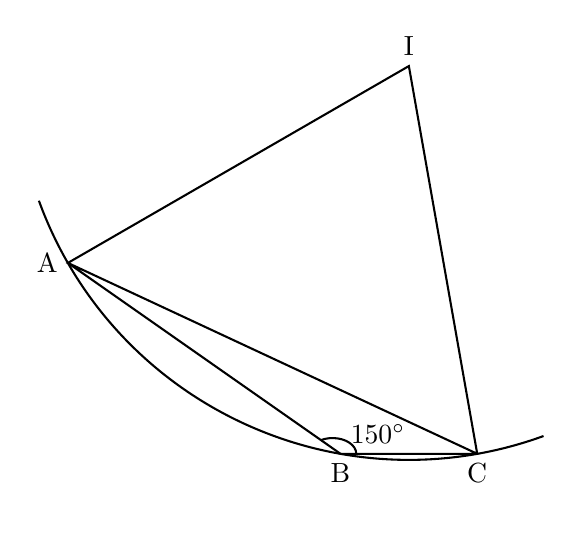
\begin{tikzpicture}
				\draw (200: 5 and 5) arc (200:290:5cm and 5cm);
				\draw (210:5 and 5) --  (260:5 and 5) --  (280:5 and 5) -- (0,0)--  (210:5 and 5) --  (280:5 and 5) ;
				\node[above] at (0,0) {I};
				\node[above right] at (260:5 and 5) {$150^\circ$};
				\node[left] at (210:5 and 5) {A};
				\node[below] at (260:5 and 5) {B};
				\node[below] at (280:5 and 5) {C};
				\draw (0.2,0)+(260: 5 and 5) arc (0:120:0.3cm and 0.2cm);
			\end{tikzpicture}
		\end{center}
		Giả sử mặt đáy trên của hình trụ là đường tròn tâm $ I$, bán kính $ R$ đi qua ba điểm $ A$, $ B$, $ C$ như hình vẽ.\\
		Khi đó $ 2R=\dfrac{AC}{\sin\widehat{ABC}}=\dfrac{4,45}{\sin 150^\circ}\Rightarrow R=4,45$ m.\\
		Thế nên $\Delta IAC$ là tam giác đều.\\
		Do đó độ dài dây cung $ AC$ là $l=\alpha R=\dfrac{\pi}{3}.R=\dfrac{89}{60}\pi $ .\\
		Tấm kính khi trải phẳng ra là một hình chữ nhật có chiều rộng là $ 1,35$ m và chiều dài $\dfrac{89}{60}\pi $ m.\\
		Thế nên số tiền ông Bình mua tấm kính trên là $1500000\cdot 1,35\cdot \dfrac{89}{60}\pi\approx 9.437.000$ đồng.
	}
\end{ex}

\begin{ex}%Câu 27 [2H2B1-2]
	Một công ty sản xuất bồn đựng nước hình trụ có thể tích thực $1$ m$^3$ với chiều cao bằng $ 1$ m. Biết bề mặt xung quanh bồn được sơn bởi loại sơn màu xanh tô như hình vẽ và màu trắng là phần còn lại của mặt xung quanh; với mỗi mét vuông bề mặt lượng sơn tiêu hao $ 0,5$ lít sơn. Công ty cần sơn $10000$ bồn thì dư kiến cần bao nhiêu lít sơn màu xanh gần với số nào nhất, biết khi đo được dây cung $ BF=1$ m.
	\begin{center}
		\begin{tikzpicture}
			\draw (0,0) ellipse (2cm and 0.6cm);
			\draw (-2,0) -- (-2,-4);
			\draw (2,0) -- (2,-4);
			\fill[cyan!30!white, smooth] (-120:2cm and 0.6cm) -- (-120:2cm and 0.6cm) arc (-120:0:2cm and 0.6cm) -- ($(0,-4)+(0:2 and 0.6)$) -- ($(0,-4)+(0:2 and 0.6)$) arc (0:-120:2cm and 0.6cm)  --  cycle;
			\draw (-2,-4) arc (180:360:2cm and 0.6cm);
			\node[draw,fill,circle,inner sep=1pt,label={-100:$B$}] (B) at (-120:2cm and 0.6cm) {};
			\node[draw,fill,circle,inner sep=1pt,label={90:$F$}] (F) at (0:2cm and 0.6cm) {};
			\node[draw,fill,circle,inner sep=1pt,label={-90:$A$}] at ($(0,-4)+(-120:2 and 0.6)$) {};
			\node[draw,fill,circle,inner sep=1pt,label={30:$E$}] at ($(0,-4)+(0:2 and 0.6)$) {};
			\draw (-120:2cm and 0.6cm) -- ($(0,-4)+(-120:2 and 0.6)$);
			\draw[dashed] (2,-4) arc (0:180:2cm and 0.6cm) (0,0)--(0,-4);
			\draw (B)--(F);
				\fill (0,0) circle (1.5pt);
			\fill (0,-4) circle (1.5pt);
			\node[above] at (0,0) {$O$};
			\node[below] at (0,-4) {$O'$};
		\end{tikzpicture}
	\end{center}
	\choice
	{\True $ 6150$}
	{$ 6250$}
	{$ 1230$}
	{$ 1250$}
	\loigiai{
		Gọi $ r$ là bán kính đường tròn đáy,\\
		Ta có: $ V=\pi{r^2}.h\Leftrightarrow r=\dfrac{1}{\sqrt{\pi}}$\\
		Xét tam giác $O'BF$ ta có $\cos(B{O}'F)=\dfrac{2r^2-B{F^2}}{2r^2}=1-\dfrac{\pi}{2}\Rightarrow\widehat{B{O}'F}\approx 2,178271695$ (rad)\\
		Vậy độ dài cung $ BF$: $ l=r\cdot \alpha\approx 1,2289582$ (m)\\
		Tổng số lít sơn màu xanh cho mỗi bồn nước là: $ T=l\cdot 0,5=0,6144791001$ (lít)\\
		Vậy tổng số sơn cần cho $ 10000$ bồn $ S\approx 6145$ (lít)\\}
\end{ex}

\begin{dang}
	{Thể tích}
\end{dang}
%%%%---1-11-D2----
\begin{ex}%Câu 1 %[2H2K1-1]%
	Cho hình trụ có chiều cao bằng $6a$. Biết rằng khi cắt hình trụ đã cho bởi một mặt phẳng song song với trục và cách trục một khoảng bằng $3a$, thiết diện thu được là một hình vuông. Thể tích của khối trụ được giới hạn bởi hình trụ đã cho bằng
	\choice
	{$216\pi a^3$}
	{$150\pi a^3$}
	{$54\pi a^3$}
	{$\True108\pi a^3$}
	\loigiai
	{\begin{center}
			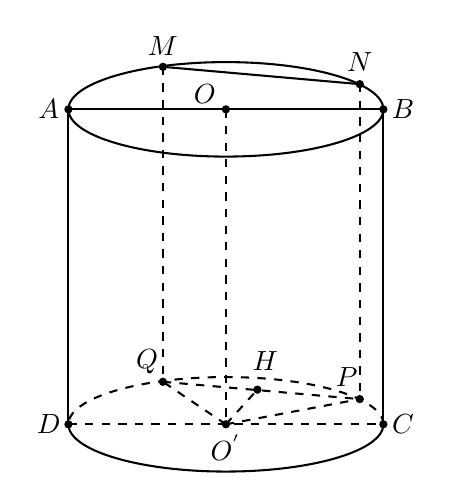
\begin{tikzpicture}
				\draw (0,0) ellipse (2cm and 0.6cm);
				\draw (-2,0) -- (-2,-4);
				\draw (2,0) -- (2,-4);
				\draw (-2,-4) arc (180:360:2cm and 0.6cm);
				\draw[dashed] (2,-4) arc (0:180:2cm and 0.6cm);
				\node[left] at (0,0.2) {\normalsize$O$};
				\fill (0,0) circle (1.5pt);
				\node[below] at (0,-4) {\normalsize$O^{'}$};
				\fill (0,-4) circle (1.5pt);
				\draw[dashed] (0,0) -- (0,-4);
				\fill (2,0) circle (1.5pt);
				\node at (-2.25,0) {\normalsize$A$};
				\fill (-2,0) circle (1.5pt);
				\node at (2.25,0) {\normalsize$B$};
				\draw (-2,0) -- (2,0);
				\fill (2,-4) circle (1.5pt);
				\node at (-2.25,-4) {\normalsize$D$};
				\fill (-2,-4) circle (1.5pt);
				\node at (2.25,-4) {\normalsize$C$};
				\draw[dashed] (-2,-4) -- (2,-4);
				\fill (1.7,0.32) circle (1.5pt);
				\fill (1.7,-3.68) circle (1.5pt);
				\draw[dashed] (1.7,0.32) -- (1.7,-3.68);
				\fill (-0.8,0.54) circle (1.5pt);
				\fill (-0.8,-3.46) circle (1.5pt);
				\draw[dashed] (-0.8,0.54) -- (-0.8,-3.46);
				\draw (-0.8,0.54) -- (1.7,0.32);
				\draw[dashed] (-0.8,-3.46) -- (1.7,-3.68);
				\draw[dashed] (0,-4) -- (-0.8,-3.46);
				\draw[dashed] (0,-4) -- (1.7,-3.68);
				\fill (0.4,-3.56) circle (1.5pt);
				\draw[dashed] (0,-4) -- (0.4,-3.56);
				\node at (1.7,0.6) {\normalsize$N$};
				\node at (-0.8,0.8) {\normalsize$M$};
				\node[left] at (1.8,-3.4) {\normalsize$P$};
				\node at (-1,-3.2) {\normalsize$Q$};
				\node at (0.5,-3.2) {\normalsize$H$};
			\end{tikzpicture}
		\end{center}
		Lấy 2 điểm $M,N$ lần lượt nằm trên đường tròn tâm $O$ sao cho $MN=6a$.\\
		Từ $M,N$ lần lượt kẻ các đường thẳng song song với trục $OO^{'}$, cắt đường tròn tâm $O^{'}$ tại $Q$ và $P$.\\
		Thiết diện thu được là hình vuông $MNPQ$ có cạnh bằng $6a$.\\
		Gọi $H$ là trung điểm của $PQ$. Suy ra $OH \perp PQ$.\\
		Vì $OO^{'} \parallel (MNPQ)$ nên ta có $\mathrm{\,d}(OO^{'},(MNPQ))=\mathrm{\,d}(O^{'},(MNPQ))=O^{'}H$.\\
		Từ giả thiết, ta có $O^{'}H=3a$. Do đó $\Delta O^{'}HP$ là tam giác vuông cân tại $H$.\\
		Suy ra bán kính đường tròn đáy của hình trụ là $O^{'}P=\sqrt{O^{'}H^{2}+HP^{2}}=3a\sqrt{2}$.\\
		Vậy thể tích khối trụ cần tìm là $V=6a \pi \left(3a\sqrt{2}\right)^2=108\pi a^3$.}
\end{ex}
\begin{ex} %Câu 2 %[2H2K1-1]%
	Một khối đồ chơi gồm hai khối trụ $(H_1),(H_2)$ xếp chồng lên nhau, lần lượt có bán kính đáy và chiều cao tương ứng là $r_1,h_1,r_2,h_2$ thỏa mãn $r_2=\dfrac{1}{2}r_1,h_2=2h_1$ (tham khảo hình vẽ). Biết rằng thể tích của toàn bộ khối đồ chơi bằng $30 \text{cm}^3$, thể tích khối trụ $(H_1)$ bằng
	\begin{center}
		\tikzset{every picture/.style={line width=0.75pt}}
		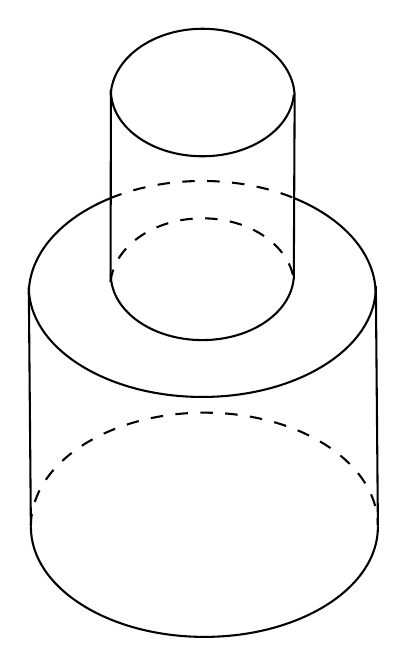
\begin{tikzpicture}[x=0.75pt,y=0.75pt,yscale=-1,xscale=1]
			\draw  [draw opacity=0][dash pattern={on 4.5pt off 4.5pt}] (259.8,244.37) .. controls (259.8,244.29) and (259.8,244.21) .. (259.8,244.13) .. controls (259.77,214.04) and (297.17,189.61) .. (343.33,189.57) .. controls (389.28,189.53) and (426.6,213.68) .. (426.95,243.59) -- (343.38,244.06) -- cycle ; \draw  [dash pattern={on 4.5pt off 4.5pt}] (259.8,244.37) .. controls (259.8,244.29) and (259.8,244.21) .. (259.8,244.13) .. controls (259.77,214.04) and (297.17,189.61) .. (343.33,189.57) .. controls (389.28,189.53) and (426.6,213.68) .. (426.95,243.59) ;  
			\draw  [draw opacity=0] (427,244.37) .. controls (427,244.44) and (427,244.52) .. (427,244.6) .. controls (427,273.87) and (389.57,297.6) .. (343.4,297.6) .. controls (297.23,297.6) and (259.8,273.87) .. (259.8,244.6) .. controls (259.8,244.52) and (259.8,244.44) .. (259.8,244.37) -- (343.4,244.6) -- cycle ; \draw   (427,244.37) .. controls (427,244.44) and (427,244.52) .. (427,244.6) .. controls (427,273.87) and (389.57,297.6) .. (343.4,297.6) .. controls (297.23,297.6) and (259.8,273.87) .. (259.8,244.6) .. controls (259.8,244.52) and (259.8,244.44) .. (259.8,244.37) ;  
			\draw  [draw opacity=0] (426,128.77) .. controls (426,128.84) and (426,128.92) .. (426,129) .. controls (426,158.27) and (388.57,182) .. (342.4,182) .. controls (296.23,182) and (258.8,158.27) .. (258.8,129) .. controls (258.8,128.92) and (258.8,128.84) .. (258.8,128.77) -- (342.4,129) -- cycle ; \draw   (426,128.77) .. controls (426,128.84) and (426,128.92) .. (426,129) .. controls (426,158.27) and (388.57,182) .. (342.4,182) .. controls (296.23,182) and (258.8,158.27) .. (258.8,129) .. controls (258.8,128.92) and (258.8,128.84) .. (258.8,128.77) ;  
			\draw  [draw opacity=0] (386.41,124.96) .. controls (384.93,141.51) and (365.79,154.6) .. (342.4,154.6) .. controls (318.04,154.6) and (298.3,140.41) .. (298.3,122.9) .. controls (298.3,122.86) and (298.3,122.82) .. (298.3,122.78) -- (342.4,122.9) -- cycle ; \draw   (386.41,124.96) .. controls (384.93,141.51) and (365.79,154.6) .. (342.4,154.6) .. controls (318.04,154.6) and (298.3,140.41) .. (298.3,122.9) .. controls (298.3,122.86) and (298.3,122.82) .. (298.3,122.78) ;  
			\draw  [draw opacity=0][dash pattern={on 4.5pt off 4.5pt}] (298.2,126.55) .. controls (299.89,109.45) and (319.01,95.96) .. (342.37,95.93) .. controls (365.24,95.91) and (384.07,108.82) .. (386.47,125.4) -- (342.4,129) -- cycle ; \draw  [dash pattern={on 4.5pt off 4.5pt}] (298.2,126.55) .. controls (299.89,109.45) and (319.01,95.96) .. (342.37,95.93) .. controls (365.24,95.91) and (384.07,108.82) .. (386.47,125.4) ;  
			\draw    (258.8,128.77) -- (259.8,244.37) ;
			\draw    (426,128.77) -- (427,244.37) ;
			\draw  [draw opacity=0] (386.47,36.4) .. controls (384.99,52.95) and (365.85,66.04) .. (342.46,66.04) .. controls (318.1,66.04) and (298.36,51.85) .. (298.36,34.34) .. controls (298.36,34.3) and (298.36,34.26) .. (298.36,34.22) -- (342.46,34.34) -- cycle ; \draw   (386.47,36.4) .. controls (384.99,52.95) and (365.85,66.04) .. (342.46,66.04) .. controls (318.1,66.04) and (298.36,51.85) .. (298.36,34.34) .. controls (298.36,34.3) and (298.36,34.26) .. (298.36,34.22) ;  
			\draw  [draw opacity=0] (298.26,36.61) .. controls (299.02,18.85) and (318.55,4.62) .. (342.53,4.6) .. controls (367,4.58) and (386.85,19.35) .. (386.89,37.6) -- (342.56,37.67) -- cycle ; \draw   (298.26,36.61) .. controls (299.02,18.85) and (318.55,4.62) .. (342.53,4.6) .. controls (367,4.58) and (386.85,19.35) .. (386.89,37.6) ;  
			\draw    (298.36,34.22) -- (298.2,126.55) ;
			\draw    (386.89,37.6) -- (386.47,125.4) ;
			\draw  [draw opacity=0][dash pattern={on 4.5pt off 4.5pt}] (297.82,86.35) .. controls (310.71,81.04) and (325.97,77.96) .. (342.33,77.94) .. controls (358.22,77.93) and (373.07,80.81) .. (385.73,85.82) -- (342.38,132.43) -- cycle ; \draw  [dash pattern={on 4.5pt off 4.5pt}] (297.82,86.35) .. controls (310.71,81.04) and (325.97,77.96) .. (342.33,77.94) .. controls (358.22,77.93) and (373.07,80.81) .. (385.73,85.82) ;  
			\draw  [draw opacity=0] (258.78,132.75) .. controls (258.78,132.67) and (258.78,132.59) .. (258.78,132.52) .. controls (258.76,113.08) and (274.35,96.01) .. (297.82,86.35) -- (342.35,132.44) -- cycle ; \draw   (258.78,132.75) .. controls (258.78,132.67) and (258.78,132.59) .. (258.78,132.52) .. controls (258.76,113.08) and (274.35,96.01) .. (297.82,86.35) ;  
			\draw  [draw opacity=0] (386.31,86.06) .. controls (409.91,95.59) and (425.7,112.57) .. (425.93,131.98) -- (342.35,132.44) -- cycle ; \draw   (386.31,86.06) .. controls (409.91,95.59) and (425.7,112.57) .. (425.93,131.98) ;  
		\end{tikzpicture}
	\end{center}
	\choice
	{$24 \text{cm}^3$}
	{$15 \text{cm}^3$}
	{$\True20 \text{cm}^3$}
	{$10 \text{cm}^3$}
	\loigiai
	{Gọi $V_1,V_2$ lần lượt là thể tích khối trụ $(H_1),(H_2)$.\\
		Ta có: $V_2=\pi r_2^2h_2=\pi{\left(\dfrac{1}{2}{r_1}\right)^2}2h_1=\dfrac{V_1}{2}$.\\
		$\Rightarrow{V_1}=2V_2$ mà $V_1+V_2=30\Rightarrow{V_1}=20$.}
\end{ex}
\begin{ex} %Câu 3 %[2H2K1-1]%
	Cho hình trụ có chiều cao bằng $8a$. Biết hai điểm $A,C$ lần lượt nằm trên hai đáy thỏa $AC=10a$, khoảng cách giữa $AC$ và trục của hình trụ bằng $4a$. Thể tích khối trụ đã cho là
	\choice
	{$128\pi a^3$}
	{$320\pi a^3$}
	{$80\pi a^3$}
	{$\True200\pi a^3$}
	\loigiai
	{\begin{center}
			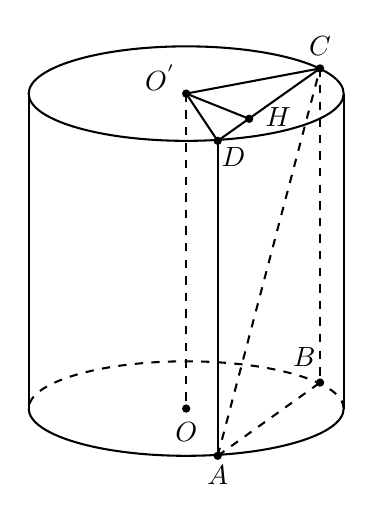
\begin{tikzpicture}
				\draw (0,0) ellipse (2cm and 0.6cm);
				\draw (-2,0) -- (-2,-4);
				\draw (2,0) -- (2,-4);
				\draw (-2,-4) arc (180:360:2cm and 0.6cm);
				\draw[dashed] (2,-4) arc (0:180:2cm and 0.6cm);
				\node[left] at (0,0.2) {\normalsize$O^{'}$};
				\fill (0,0) circle (1.5pt);
				\node at (0,-4.3) {\normalsize$O$};
				\draw[dashed] (0,0) -- (0,-4);
				\fill (0,-4) circle (1.5pt);
				\fill (1.7,0.32) circle (1.5pt);
				\node at (1.7,0.6) {\normalsize$C$};
				\fill (1.7,-3.67) circle (1.5pt);
				\node at (1.5,-3.35) {\normalsize$B$};
				\fill (0.4,-0.6) circle (1.5pt);
				\node at (0.6,-0.8) {\normalsize$D$};
				\fill (0.4,-4.6) circle (1.5pt);
				\node at (0.4,-4.85) {\normalsize$A$};
				\fill (0.8,-0.32) circle (1.5pt);
				\node at (1.17,-0.3) {\normalsize$H$};
				\draw[dashed] (1.7,0.32) -- (1.7,-3.67);
				\draw[dashed] (0.4,-4.6) -- (1.7,-3.67);
				\draw (0.4,-4.6) -- (0.4,-0.6);
				\draw (0.4,-0.6) -- (1.7,0.32);
				\draw[dashed] (0.4,-4.6) -- (1.7,0.32);
				\draw (0,0) -- (1.7,0.32);
				\draw (0,0) -- (0.4,-0.6);
				\draw (0,0) -- (0.8,-0.32);
			\end{tikzpicture}
		\end{center}
		Gọi $(O),\left(O'\right)$ lần lượt là hai đường tròn đáy. $ A\in(O),C\in\left(O'\right)$.\\
		Dựng $AD,CB$ lần lượt song song với $ O{O}'$$(D\in\left(O'\right),B\in(O))$. Dễ dàng có $ ABCD$ là hình chữ nhật.\\
		Do $ AC=10a,AD=8a\Rightarrow DC=6a$.\\
		Gọi $ H$ là trung điểm của $ DC$.\\
		$\left\{\begin{matrix}
			{O}'H\perp DC\\
			{O}'H\perp AD\\
		\end{matrix}\right.\Rightarrow{O}'H\perp\left(ABCD\right)$.\\
		Ta có $ O{O}'\parallel\left(ABCD\right)$$\Rightarrow d\left(O{O}',AC\right)=d\left(O{O}',\left(ABCD\right)\right)=O'H=4a$.\\
		$O'H=4a,CH=3a\Rightarrow R=O'C=5a$.\\
		Vậy thể tích của khối trụ là $ V=\pi{R^2}h=\pi{\left(5a\right)^2}8a=200\pi{a^3}$.}
\end{ex}
\begin{ex} %Câu 4 %[2H2K1-1]%
	Hỏi nếu tăng chiều cao của khối trụ lên 2 lần, bán kính của nó lên 3 lần thì thể tích của khối trụ mới sẽ tăng bao nhiêu lần so với khối trụ ban đầu?
	\choice
	{$36$}
	{$6$}
	{\True$18$}
	{$12$}
	\loigiai
	{Giả sử ban đầu khối trụ có chiều cao $h_1$ và bán kính $r_1$.\\
		Khi đó, khối trụ có thể tích là $V_1=\pi r_1^2h$.\\
		Sau khi tăng chiều cao của khối trụ lên $ 2$ lần, bán kính của nó lên $3$ lần thì khối trụ có chiều cao $ 2h_1$ và bán kính $3r_1$.\\
		Khi đó, khối trụ mới có thể tích là $V_2=\pi{\left(3r_1\right)^2}\cdot2h_1=18\pi{r_1}{h_1}$.\\
		Do vậy $\dfrac{V_2}{V_1}=18$.}
\end{ex}
\begin{ex} %Câu 5 %[2H2K1-1]%
	Cần đẽo thanh gỗ hình hộp có đáy là hình vuông thành hình trụ có cùng chiều cao. Tỉ lệ thể tích gỗ cần phải đẽo đi ít nhất (tính gần đúng) là
	\choice
	{$30\%$}
	{$50\%$}
	{\True$21\%$}
	{$11\%$}
	\loigiai
	{
		\begin{center}     
			\tikzset{every picture/.style={line width=0.75pt}}
			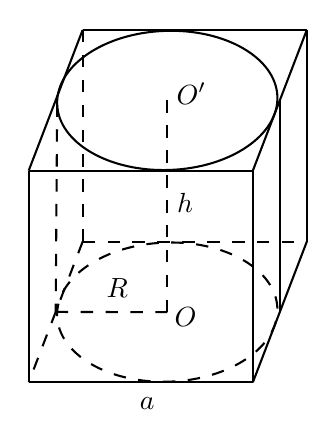
\begin{tikzpicture}[x=0.75pt,y=0.75pt,yscale=-1,xscale=1]
				\draw  [dash pattern={on 4.5pt off 4.5pt}]  (164,221.2) -- (138,289) ;
				\draw    (272,221.2) -- (246,289) ;
				\draw  [dash pattern={on 4.5pt off 4.5pt}]  (164,221.2) -- (272,221.2) ;
				\draw    (138,289) -- (246,289) ;
				\draw    (164,119.2) -- (272,119.2) ;
				\draw    (138,187) -- (246,187) ;
				\draw    (164,119.2) -- (138,187) ;
				\draw    (272,119.2) -- (246,187) ;
				\draw    (138,187) -- (138,289) ;
				\draw  [dash pattern={on 4.5pt off 4.5pt}]  (164,119.2) -- (164,221.2) ;
				\draw    (246,187) -- (246,289) ;
				\draw    (272,119.2) -- (272,221.2) ;
				\draw   (151.7,155.08) .. controls (151.04,136.58) and (174.26,120.73) .. (203.56,119.69) .. controls (232.86,118.64) and (257.15,132.8) .. (257.81,151.3) .. controls (258.47,169.8) and (235.25,185.65) .. (205.94,186.69) .. controls (176.64,187.73) and (152.35,173.58) .. (151.7,155.08) -- cycle ;
				\draw  [dash pattern={on 4.5pt off 4.5pt}] (151.7,257.08) .. controls (151.04,238.58) and (174.26,222.73) .. (203.56,221.69) .. controls (232.86,220.64) and (257.15,234.8) .. (257.81,253.3) .. controls (258.47,271.8) and (235.25,287.65) .. (205.94,288.69) .. controls (176.64,289.73) and (152.35,275.58) .. (151.7,257.08) -- cycle ;
				\draw  [dash pattern={on 4.5pt off 4.5pt}]  (151.7,155.08) -- (151,255.1) ;
				\draw    (259,153.1) -- (259,255.1) ;
				\draw  [dash pattern={on 4.5pt off 4.5pt}]  (204.75,153.19) -- (204.75,255.19) ;
				\draw  [dash pattern={on 4.5pt off 4.5pt}]  (151,255.1) -- (204.75,255.19) ;
				\draw (206.75,251.59) node [anchor=north west][inner sep=0.75pt]    {$O$};
				\draw (207.75,143.4) node [anchor=north west][inner sep=0.75pt]    {$O'$};
				\draw (190,295) node [anchor=north west][inner sep=0.75pt]    {$a$};
				\draw (174,237.4) node [anchor=north west][inner sep=0.75pt]    {$R$};
				\draw (208,196.4) node [anchor=north west][inner sep=0.75pt]    {$h$};
			\end{tikzpicture}
		\end{center}
		Để gỗ bị đẽo ít nhất thì hình hộp đó phải là hình hộp đứng.\\
		Gọi $ h$ là chiều cao của hình hộp chữ nhật và $ R$ là bán kính đáy của hình trụ.\\
		Do hình hộp chữ nhật và hình trụ có cùng chiều cao nên thể tích gỗ đẽo đi ít nhất khi và chỉ khi diện tích đáy của hình trụ lớn nhất (thể tích khối trụ lớn nhất). Suy ra $ R=\dfrac{a}{2}$.\\
		Gọi $V_1$ và $V_2$ lần lượt là thể tích của khối hộp và thể tích của khối trụ có đáy lớn nhất.\\
		Ta có: $V_1=a^2\cdot h$ và $V_2=\pi{R^2}\cdot h=\pi\cdot\dfrac{a^2}{4}\cdot h$.\\
		Suy ra: $\dfrac{V_2}{V_1}=\dfrac{\pi\cdot\dfrac{a^2}{4}\cdot h}{a^2\cdot h}=\dfrac{\pi}{4}\approx 78{,}54\%$.\\
		Vậy thể tích gỗ ít nhất cần đẽo đi là khoảng $21{,}46\%$.}
\end{ex}
\begin{ex} %Câu 6 %[2H2K1-1]%
	Một khối gỗ hình trụ có đường kính $0{,}5\text{m}$ và chiều cao $1\text{m}$. Người ta đã cắt khối gỗ, phần còn lại như hình vẽ bên có thể tích là $V$. Tính $V$.
	\begin{center}
		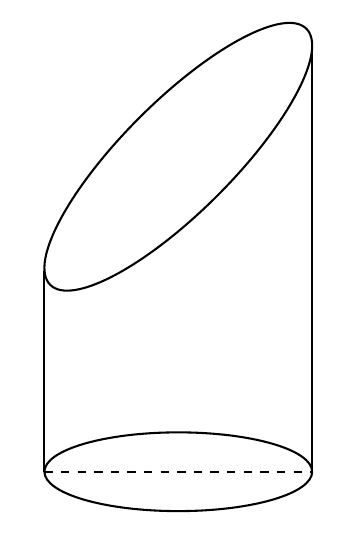
\begin{tikzpicture}
			\draw[rotate=45] (0,0) ellipse (2.3cm and 0.7cm);
			\draw (-1.7,-1.45) -- (-1.7,-4);
			\draw (1.7,1.45) -- (1.7,-4);
			\draw (0,-4) ellipse (1.7cm and 0.5cm);
			\draw[dashed] (-1.7,-4) -- (1.7,-4);
		\end{tikzpicture}
	\end{center}
	\choice
	{$\dfrac{3\pi}{16}$$\left(\text{m}^3\right)$}
	{$\dfrac{5\pi}{64}$$\left(\text{m}^3\right)$}
	{\True $\dfrac{3\pi}{64}$$\left(\text{m}^3\right)$}
	{$\dfrac{\pi}{16}$$\left(\text{m}^3\right)$}
	\loigiai
	{Gọi $V_1$, $V_2$ lần lượt là thể tích khối gỗ ban đầu và thể tích khối gỗ bị cắt.\\
		Thể tích của khối gỗ ban đầu là $V_1=\pi{\left(\dfrac{0{,}5}{2}\right)^2}\cdot 1=\dfrac{\pi}{16}$$\left(\text{m}^3\right)$.\\
		Thể tích phần gỗ đã bị cắt đi là $V_2=\dfrac{1}{2}\pi{\left(\dfrac{0{,}5}{2}\right)^2}\cdot0{,}5=\dfrac{\pi}{64}$$\left(\text{m}^3\right)$.\\
		Thể tích khối gỗ còn lại và $ V=V_1-V_2=\dfrac{\pi}{16}-\dfrac{\pi}{64}=\dfrac{3\pi}{64}$$\left(\text{m}^3\right)$.}
\end{ex}
\begin{ex}%Câu 7 %[2H2K1-1]%
	Cho hình trụ có $ O,\,O'$ là tâm hai đáy. Xét hình chữ nhật $ ABCD$ có $ A,\,B$ cùng thuộc $(O)$ và $ C,\,D$ cùng thuộc $\left(O'\right)$ sao cho $ AB=a\sqrt{3}$, $ BC=2a$ đồng thời $\left(ABCD\right)$ tạo với mặt phẳng đáy hình trụ góc $ 60^\circ $. Thể tích khối trụ bằng
	\choice
	{\True $\pi{a^3}\sqrt{3}$}
	{$\dfrac{\pi{a^3}\sqrt{3}}{9}$}
	{$\dfrac{\pi{a^3}\sqrt{3}}{3}$}
	{$ 2\pi{a^3}\sqrt{3}$}
	\loigiai
	{\begin{center}
			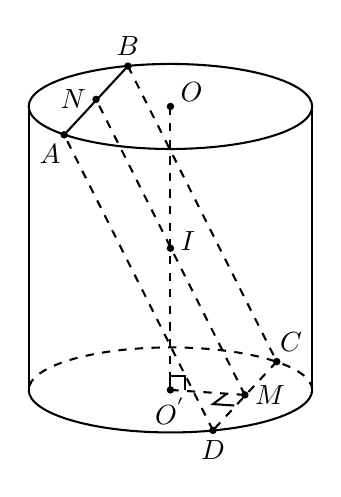
\begin{tikzpicture}[scale=0.9]
				\draw (0,0) ellipse (2cm and 0.6cm);
				\draw (-2,0) -- (-2,-4);
				\draw (2,0) -- (2,-4);
				\draw (-2,-4) arc (180:360:2cm and 0.6cm);
				\draw[dashed] (2,-4) arc (0:180:2cm and 0.6cm);
				\node[right] at (0,0.2) {\normalsize$O$};
				\fill (0,0) circle (1.5pt);
				\node at (0,-4.3) {\normalsize$O^{'}$};
				\draw[dashed] (0,0) -- (0,-4);
				\fill (0,-4) circle (1.5pt);
				\fill (-0.6,0.57) circle (1.5pt);
				\fill (-1.5,-0.4) circle (1.5pt);
				\draw (-0.6,0.57) -- (-1.5,-0.4);
				\fill (-1.05,0.1) circle (1.5pt);
				\fill (1.5,-3.6) circle (1.5pt);
				\fill (0.6,-4.57) circle (1.5pt);
				\fill (1.05,-4.07) circle (1.5pt);
				\draw[dashed] (-0.6,0.57) -- (1.5,-3.6);
				\draw[dashed] (0.6,-4.57) -- (-1.5,-0.4);
				\draw[dashed] (1.5,-3.6) -- (0.6,-4.57);
				\draw[dashed] (1.05,-4.07) -- (-1.05,0.1);
				\draw[dashed] (1.05,-4.07) -- (0,-4);
				\draw (0,-4) -- (0,-3.8) -- (0.2,-3.8) -- (0.2,-4);
				\draw (0.8,-4.05) -- (0.6,-4.2) -- (0.9,-4.22);
				\fill (0,-2) circle (1.5pt);
				\node[above] at (-0.6,0.57) {\normalsize$B$};
				\node[below] at (-1.7,-0.4) {\normalsize$A$};
				\node[left] at (-1.05,0.1) {\normalsize$N$};
				\node[right] at (0,-1.9) {\normalsize$I$};
				\node[above] at (1.7,-3.6) {\normalsize$C$};
				\node[below] at (0.6,-4.57) {\normalsize$D$};
				\node[right] at (1.05,-4.07) {\normalsize$M$};
			\end{tikzpicture}
		\end{center}
		Gọi $ M,\,N$ lần lượt là trung điểm của $ CD,\,AB$ và $ I$ là trung điểm của $O{O}'$ .\\
		Suy ra góc giữa mặt phẳng $\left(ABCD\right)$ và mặt phẳng đáy là $\widehat{IM{O}'}=60^\circ $.\\
		Ta có $ IM=\dfrac{1}{2}MN=\dfrac{1}{2}BC=a$.\\
		Xét $\Delta I{O}'M$ vuông tại $ O$, ta có $ I{O}'=IM\cdot\sin\widehat{IM{O}'}=\dfrac{a\sqrt{3}}{2}\Rightarrow h=O{O}'=2I{O}'=a\sqrt{3}$;\\
		$O'M=IM\cdot\cos\widehat{IM{O}'}=\dfrac{a}{2}$.\\
		Xét $\Delta{O}'MD$ vuông tại $ M$, có $O'M=\dfrac{a}{2},\,MD=\dfrac{1}{2}CD=\dfrac{1}{2}AB=\dfrac{a\sqrt{3}}{2}$.\\
		$\Rightarrow r=O'D=\sqrt{O^{'}{M^2}+M{D^2}}=\sqrt{\left(\dfrac{a}{2}\right)^2+\left(\dfrac{a\sqrt{3}}{2}\right)^2}\Rightarrow r=a$.\\
		Vậy $ V=\pi{r^2}h=\pi{a^3}\sqrt{3}$.}
\end{ex}
\begin{ex}%Câu 8 %[2H2K1-1]%
	Cho khối trụ có hai đáy là $(O)$ và $\left(O'\right)$. $AB,CD$ lần lượt là hai đường kính của $(O)$ và $\left(O'\right)$, góc giữa $AB$ và $CD$ bằng $30^\circ $, $AB=6$. Thể tích khối tứ diện $ABCD$ bằng $30$. Thể tích khối trụ đã cho bằng
	\choice
	{$180\pi$}
	{\True $90\pi$}
	{$30\pi$}
	{$45\pi$}
	\loigiai
	{	\begin{center}
			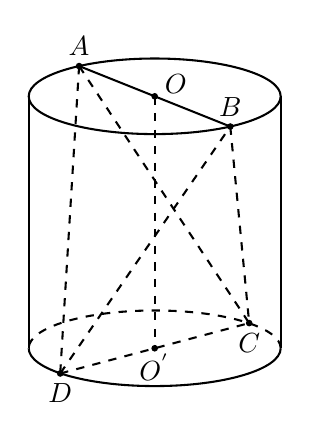
\begin{tikzpicture}[scale=0.8]
				\draw (0,0) ellipse (2cm and 0.6cm);
				\draw (-2,0) -- (-2,-4);
				\draw (2,0) -- (2,-4);
				\draw (-2,-4) arc (180:360:2cm and 0.6cm);
				\draw[dashed] (2,-4) arc (0:180:2cm and 0.6cm);
				\node[right] at (0,0.2) {\normalsize$O$};
				\fill (0,0) circle (1.5pt);
				\node at (0,-4.3) {\normalsize$O^{'}$};
				\draw[dashed] (0,0) -- (0,-4);
				\fill (0,-4) circle (1.5pt);
				\fill (-1.2,0.48) circle (1.5pt);
				\node[above] at (-1.2,0.48) {\normalsize$A$};
				\fill (1.2,-0.48) circle (1.5pt);
				\node[above] at (1.2,-0.48) {\normalsize$B$};
				\draw (-1.2,0.48) -- (1.2,-0.48);
				\fill (1.5,-3.6) circle (1.5pt);
				\node[below] at (1.5,-3.6) {\normalsize$C$};
				\fill (-1.5,-4.4) circle (1.5pt);
				\node[below] at (-1.5,-4.4) {\normalsize$D$};
				\draw[dashed] (-1.5,-4.4) -- (1.5,-3.6);
				\draw[dashed] (-1.2,0.48) -- (-1.5,-4.4);
				\draw[dashed] (1.2,-0.48) -- (1.5,-3.6);
				\draw[dashed] (-1.2,0.48) -- (1.5,-3.6);
				\draw[dashed] (-1.5,-4.4) -- (1.2,-0.48);
			\end{tikzpicture}
		\end{center}
		Ta chứng minh: $V_{ABCD}=\dfrac{1}{6}AB\cdot CD\cdot\mathrm{\,d}\left(AB,CD\right)\cdot\sin\left(AB,CD\right)$.
		\begin{center}
			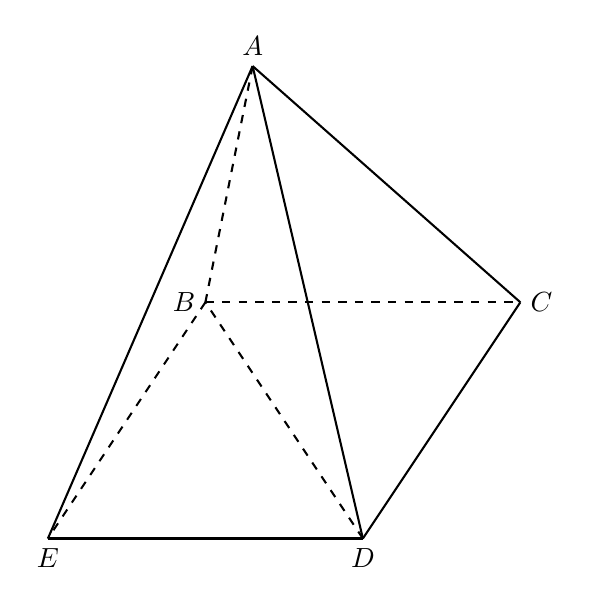
\begin{tikzpicture}[scale=2]
				\coordinate (A) at (0,0);
				\coordinate (B) at (2,0);
				\coordinate (C) at (3,1.5);
				\coordinate (D) at (1,1.5);
				\coordinate (S) at (1.3,3);
				\draw[dashed] (1,1.5) -- (1.3,3);
				\draw[dashed] (1,1.5) -- (3,1.5);
				\draw[dashed] (1,1.5) -- (0,0);
				\draw (2,0) -- (0,0);
				\draw (2,0) -- (3,1.5);
				\draw (0,0) -- (1.3,3);
				\draw (2,0) -- (1.3,3);
				\draw (3,1.5) -- (1.3,3);
				\draw[dashed] (2,0) -- (1,1.5);
				\node[below] at (0,0) {\normalsize$E$};
				\node[below] at (2,0) {\normalsize$D$};
				\node[right] at (3,1.5) {\normalsize$C$};
				\node[left] at (1,1.5) {\normalsize$B$};
				\node[above] at (1.3,3) {\normalsize$A$};
			\end{tikzpicture}
		\end{center}
		Lấy điểm $E$ sao cho tứ giác $BCDE$ là hình bình hành.\\
		Khi đó $\left(AB,CD\right)=\left(AB,BE\right)\Rightarrow\sin\left(AB,CD\right)=\sin\left(AB,BE\right)$.\\
		$\mathrm{\,d}\left(D,\,\left(ABE\right)\right)=\mathrm{\,d}\left(AB,CD\right)$.\\
		$V_{ABCD}=V_{ABDE}=\dfrac{1}{3}\cdot\mathrm{\,d}\left(D,\left(ABE\right)\right)\cdot S_{ABE}=\dfrac{1}{6}AB\cdot CD\cdot\mathrm{\,d}\left(AB,CD\right)\cdot\sin\left(AB,CD\right)$\\
		$V_{ABCD}=\dfrac{1}{6}AB\cdot CD\cdot\mathrm{\,d}\left(AB,CD\right)\cdot\sin\left(AB,CD\right)\Rightarrow \mathrm{\,d}\left(AB,CD\right)=\dfrac{6V_{ABCD}}{ABCD\cdot\sin 30^\circ}=\dfrac{180}{6\cdot6\cdot\dfrac{1}{2}}=10$.\\
		Chiều cao của lăng trụ bằng $h=d\left(AB,CD\right)=10$.\\
		Thể tích lăng trụ: $V=S\cdot h=\pi{3^2}\cdot10=90\pi$.}
\end{ex}
\begin{ex}%Câu 9 %[2H2K1-1]%
	Từ một tấm tôn hình chữ nhật có kích thước $50\text{cm} \times 240\text{cm}$, người ta làm các thùng đựng nước hình trụ có chiều cao bằng $50\text{cm}$, theo hai cách sau (xem hình minh họa dưới đây):\\
	Cách 1: Gò tấm tôn ban đầu thành mặt xung quanh thùng.\\
	Cách 2: Cắt tấm tôn ban đầu thành hai tấm bằng nhau, rồi gò mỗi tấm đó thành mặt xung quanh của một thùng.\\
	Kí hiệu $V_1$ là thể tích của thùng được gò theo cách 1 và $V_2$ là tổng thể tích của hai thùng được gò theo cách 2. Tính tỉ số $\dfrac{V_1}{V_2}$.
	\begin{center}
		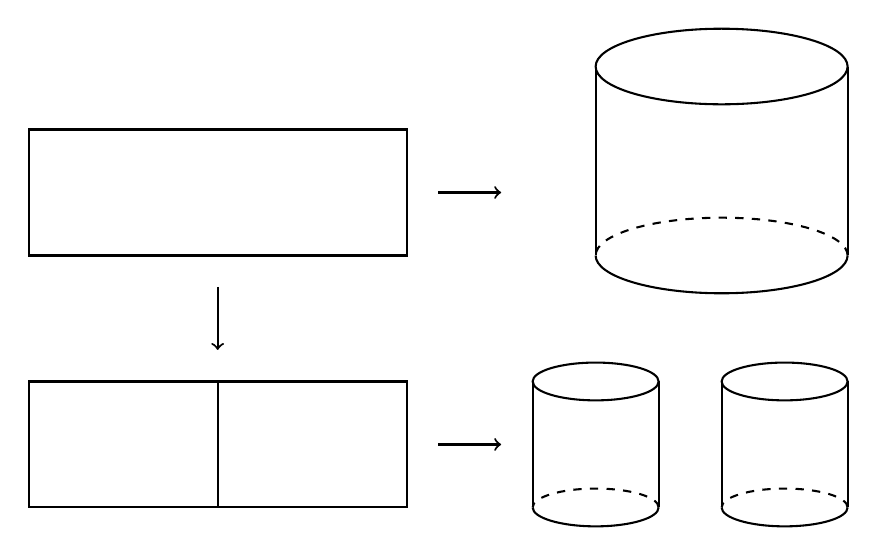
\begin{tikzpicture}[scale=0.8]
			\draw (-6,0) -- (0,0) -- (0,2) -- (-6,2) -- cycle;
			\draw[->] (-3,-0.5) -- (-3,-1.5);
			\draw (-6,-4) -- (0,-4) -- (0,-2) -- (-6,-2) -- cycle;
			\draw (-3,-2) -- (-3,-4);
			\draw[->] (0.5,1) -- (1.5,1);
			\draw[->] (0.5,-3) -- (1.5,-3);
			\draw (5,3) ellipse (2cm and 0.6cm);
			\draw (3,0) arc (180:360:2cm and 0.6cm);
			\draw[dashed] (7,0) arc (0:180:2cm and 0.6cm);
			\draw (3,3) -- (3,0);
			\draw (7,3) -- (7,0);
			\draw (3,-2) ellipse (1cm and 0.3cm);
			\draw (2,-4) arc (180:360:1cm and 0.3cm);
			\draw[dashed] (4,-4) arc (0:180:1cm and 0.3cm);
			\draw (2,-2) -- (2,-4);
			\draw (4,-2) -- (4,-4);
			\draw (6,-2) ellipse (1cm and 0.3cm);
			\draw (5,-4) arc (180:360:1cm and 0.3cm);
			\draw[dashed] (7,-4) arc (0:180:1cm and 0.3cm);
			\draw (7,-2) -- (7,-4);
			\draw (5,-2) -- (5,-4);
		\end{tikzpicture}
	\end{center}
	\choice
	{$\dfrac{V_1}{V_2}=1$}
	{$\dfrac{V_1}{V_2}=\dfrac{1}{2}$}
	{$\True\dfrac{V_1}{V_2}=2$}
	{$\dfrac{V_1}{V_2}=4$}
	\loigiai
	{Ở cách 1, thùng hình trụ có chiều cao $h=50\,\text{cm}$, chu vi đáy $C_1=240\text{cm}$ nên bán kính đáy $R_1=\dfrac{C_1}{2\pi}=\dfrac{120}{\pi}\text{cm}$. Do đó thể tích của thùng là $V_1=\pi R_1^2h$.\\
		Ở cách 2, hai thùng đều có có chiều cao $h=50\text{cm}$, chu vi đáy $C_2=120\text{cm}$ nên bán kính đáy $R_1=\dfrac{C_2}{2\pi}=\dfrac{60}{\pi}\text{cm}$. Do đó tổng thể tích của hai thùng là $V_2=2\pi R_2^2h$.\\
		Vậy $\dfrac{V_1}{V_2}=\dfrac{\pi R_1^2h}{2\pi R_2^2h}=\dfrac{1}{2}\cdot\left(\dfrac{R_1}{R_2}\right)^2=\dfrac{1}{2}\cdot\left(\dfrac{\dfrac{120}{\pi}}{\dfrac{60}{\pi}}\right)^2=2$.}
\end{ex}
\begin{ex} %Câu 10 %[2H2K1-1]%
	Cho hình trụ có hai đáy là hình tròn tâm $ O$ và $O'$, chiều cao $ h=a\sqrt{3}$. Mặt phẳng đi qua tâm $ O$ và tạo với $ O{O}'$ một góc $ 30^\circ $, cắt hai đường tròn tâm $ O$ và $O'$ tại bốn điểm là bốn đỉnh của một hình thang có đáy lớn gấp đôi đáy nhỏ và diện tích bằng $ 3a^2$. Thể tích của khối trụ được giới hạn bởi hình trụ đã cho bằng
	\choice
	{$\dfrac{\sqrt{3}\pi{a^3}}{3}$}
	{\True $\sqrt{3}\pi{a^3}$}
	{$\dfrac{\sqrt{3}\pi{a^3}}{12}$}
	{$\dfrac{\sqrt{3}\pi{a^3}}{4}$}
	\loigiai
	{	\begin{center}
			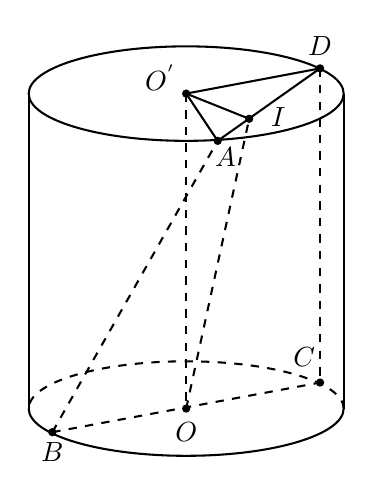
\begin{tikzpicture}
				\draw (0,0) ellipse (2cm and 0.6cm);
				\draw (-2,0) -- (-2,-4);
				\draw (2,0) -- (2,-4);
				\draw (-2,-4) arc (180:360:2cm and 0.6cm);
				\draw[dashed] (2,-4) arc (0:180:2cm and 0.6cm);
				\node[left] at (0,0.2) {\normalsize$O^{'}$};
				\fill (0,0) circle (1.5pt);
				\node at (0,-4.3) {\normalsize$O$};
				\draw[dashed] (0,0) -- (0,-4);
				\fill (0,-4) circle (1.5pt);
				\fill (1.7,0.32) circle (1.5pt);
				\node at (1.7,0.6) {\normalsize$D$};
				\fill (1.7,-3.67) circle (1.5pt);
				\node at (1.5,-3.35) {\normalsize$C$};
				\fill (0.4,-0.6) circle (1.5pt);
				\node at (0.5,-0.8) {\normalsize$A$};
				\node[below] at (-1.7,-4.3) {\normalsize$B$};
				\fill (0.8,-0.32) circle (1.5pt);
				\node at (1.17,-0.3) {\normalsize$I$};
				\draw[dashed] (1.7,0.32) -- (1.7,-3.67);
				\draw (0.4,-0.6) -- (1.7,0.32);
				\draw (0,0) -- (1.7,0.32);
				\draw (0,0) -- (0.4,-0.6);
				\draw (0,0) -- (0.8,-0.32);
				\fill (-1.7,-4.3) circle (1.5pt);
				\draw[dashed] (-1.7,-4.3) -- (1.7,-3.67);
				\draw[dashed] (-1.7,-4.3) -- (0.4,-0.6);
				\draw[dashed] (0,-4) -- (0.8,-0.32);
			\end{tikzpicture}
		\end{center}
		Giả sử $ABCD$ là hình thang mà đề bài đề cập ($BC$ là đáy lớn, $AD$ là đáy nhỏ) và $r$ là bán kính đáy của hình trụ.\\
		Theo đề: $\left\{\begin{aligned}
			& BC=2r\\ 
			& BC=2AD\\ 
		\end{aligned}\right.\Rightarrow AD=r$.\\
		Kẻ $O'I\perp AD$ $\Rightarrow AD\perp\left(O{O}'I\right)$$\Rightarrow\left(ABCD\right)\perp\left(O{O}'J\right)$.\\
		Suy ra góc giữa $O{O}'$ và $\left(ABCD\right)$ là góc $\widehat{O'OI}$. Theo đề $\widehat{O'OI}=30^\circ $.\\
		\begin{center}
			$\cos\widehat{O'OI}=\dfrac{O{O}'}{OI}\Leftrightarrow OI=\dfrac{O{O}'}{\cos 30^\circ}=\dfrac{a\sqrt{3}}{\dfrac{\sqrt{3}}{2}}=2a$.
		\end{center}
		Ta có: $S_{ABCD}=\dfrac{\left(AD+BC\right)\cdot IO}{2}\Leftrightarrow 3a^2=\dfrac{\left(r+2r\right)\cdot2a}{2}\Leftrightarrow r=a$.\\
		Thể tích của khối trụ là $V=\pi{r^2}h=\pi{a^2}\cdot a\sqrt{3}=\pi{a^3}\sqrt{3}$.}
\end{ex}
\begin{ex} %Câu 11 %[2H2K1-1]%
	Cho hình trụ và hình vuông $ ABCD$ có cạnh $ a$. Hai đỉnh liên tiếp $ A,\,B$ nằm trên đường tròn đáy thứ nhất và hai đỉnh còn lại nằm trên đường tròn đáy thức hai, mặt phẳng $\left(ABCD\right)$ tạo với đáy một góc $ 45^\circ $. Khi đó thể tích khối trụ là
	\choice
	{$\dfrac{\pi{a^3}\sqrt{2}}{8}$}
	{$\dfrac{3\pi{a^3}\sqrt{2}}{8}$}
	{$\dfrac{\pi{a^3}\sqrt{2}}{16}$}
	{\True $\dfrac{3\pi{a^3}\sqrt{2}}{16}$}
	\loigiai
	{\begin{center}
			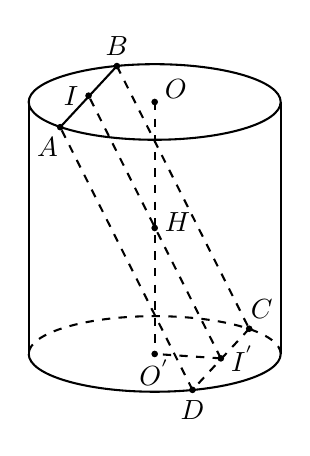
\begin{tikzpicture}[scale=0.8]
				\draw (0,0) ellipse (2cm and 0.6cm);
				\draw (-2,0) -- (-2,-4);
				\draw (2,0) -- (2,-4);
				\draw (-2,-4) arc (180:360:2cm and 0.6cm);
				\draw[dashed] (2,-4) arc (0:180:2cm and 0.6cm);
				\node[right] at (0,0.2) {\normalsize$O$};
				\fill (0,0) circle (1.5pt);
				\node at (0,-4.3) {\normalsize$O^{'}$};
				\draw[dashed] (0,0) -- (0,-4);
				\fill (0,-4) circle (1.5pt);
				\fill (-0.6,0.57) circle (1.5pt);
				\fill (-1.5,-0.4) circle (1.5pt);
				\draw (-0.6,0.57) -- (-1.5,-0.4);
				\fill (-1.05,0.1) circle (1.5pt);
				\fill (1.5,-3.6) circle (1.5pt);
				\fill (0.6,-4.57) circle (1.5pt);
				\fill (1.05,-4.07) circle (1.5pt);
				\draw[dashed] (-0.6,0.57) -- (1.5,-3.6);
				\draw[dashed] (0.6,-4.57) -- (-1.5,-0.4);
				\draw[dashed] (1.5,-3.6) -- (0.6,-4.57);
				\draw[dashed] (1.05,-4.07) -- (-1.05,0.1);
				\draw[dashed] (1.05,-4.07) -- (0,-4);
				\fill (0,-2) circle (1.5pt);
				\node[above] at (-0.6,0.57) {\normalsize$B$};
				\node[below] at (-1.7,-0.4) {\normalsize$A$};
				\node[left] at (-1.05,0.1) {\normalsize$I$};
				\node[right] at (0,-1.9) {\normalsize$H$};
				\node[above] at (1.7,-3.6) {\normalsize$C$};
				\node[below] at (0.6,-4.57) {\normalsize$D$};
				\node[right] at (1.05,-4.07) {\normalsize$I^{'}$};
			\end{tikzpicture}
		\end{center}
		Gọi $ I,\,I'$ lần lượt là trung điểm của $ AB,\,CD$; $ O,\,O'$ lần lượt là tâm đường tròn đáy của hình trụ (như hình vẽ); $ H$ là trung điểm của $ I{I}'$.\\
		Khi đó $ H$ là trung điểm của $ O{O}'$ và góc giữa $\left(ABCD\right)$ tạo với đáy là $\widehat{H{I}'O}=45^\circ $.\\
		Do $I'H=\dfrac{a}{2}$$\Rightarrow{O}'H=O'{I}'=\dfrac{a\sqrt{2}}{4}$. Khi đó $ h=O{O}'=\dfrac{a\sqrt{2}}{2}$.\\
		Ta có: $ r=O'C=\sqrt{O'{I'^2}+I'{C^2}}=\dfrac{a\sqrt{6}}{4}$.\\
		Thể tích khối trụ là $ V=\pi{r^2}h=\dfrac{3\pi{a^3}\sqrt{2}}{16}$.}
\end{ex}

\begin{dang}{Khối tròn xoay nội, ngoại tiếp khối đa diện}
\end{dang}
%%%%----1-8-D3
\begin{ex}%[2H2K1-3]%Câu 39 [Đề Tham Khảo 2018] 
	Cho tứ diện đều $ABCD$ có cạnh bằng $4$. Tính diện tích xung quanh $S_{xq}$ của hình trụ có một đường tròn đáy là đường tròn nội tiếp tam giác $BCD$ và chiều cao bằng chiều cao của tứ diện $ABCD$.
	\choice
	{$S_{xq}=8\sqrt{3}\pi $}
	{$S_{xq}=8\sqrt{2}\pi $}
	{$S_{xq}=\dfrac{16\sqrt{3}\pi}{3}$}
	{\True $S_{xq}=\dfrac{16\sqrt{2}\pi}{3}$}
	\loigiai{
		\immini{
			Bán kính hình trụ bằng $\dfrac{1}{3}$ đường cao tam giác $BCD$ nên $r=\dfrac{1}{3}\cdot\dfrac{4\sqrt{3}}{2}=\dfrac{2\sqrt{3}}{3}$.\\
			Chiều cao hình trụ bằng chiều cao hình chóp 
			$$h=\sqrt{4^2-\left(\dfrac{2}{3}\cdot\dfrac{4\sqrt{3}}{2}\right)^2}=\sqrt{16-\dfrac{16\cdot 3}{9}}=\dfrac{4\sqrt{2}}{\sqrt{3}}.$$
			Vậy $S_{xq}=2\pi rh=2\pi \cdot\dfrac{2\sqrt{3}}{3}\cdot\dfrac{4\sqrt{2}}{\sqrt{3}}=\dfrac{16\sqrt{2}\pi}{3}$.
		}{
			\begin{tikzpicture}[line join = round, line cap = round,>=stealth,font=\footnotesize,scale=0.8]
				\draw[dashed,thin] (2,0) arc (0:360:2cm and 0.6cm);
				\draw (2,4.5) arc (0:360:2cm and 0.6cm);
				\coordinate (A) at (0,4.5);
				\coordinate (B) at (-4.7,0.6);
				\coordinate (D) at (3,0.6);
				\coordinate (C) at (0.7,-1.1);
				\coordinate (O) at (0,0) ;
				\coordinate (M) at (-2,0);
				\coordinate (M') at (-2,4.5);
				\coordinate (N) at (2,0);
				\coordinate (N') at (2,4.5);
				\path
				(intersection of A--B and M--M') coordinate (H)
				(intersection of A--D and N--N') coordinate (K)
				($(A)!0.5!(C)$) coordinate (I)
				;
				\draw (M')--(H)--(B)--(C)--(D)--(K)--(N') (C)--(I);
				\draw[dashed] (M)--(H) (N)--(K) (B)--(D) (H)--(A)--(I) (B)--(O)--(A)--(K);
				\foreach \x/\g in {O/-90,A/90,B/-100,C/-50,D/-40}\fill[black](\x)circle(1pt)+(\g:.3)node{$\x$} ;
			\end{tikzpicture}
		}
	}
\end{ex}

\begin{ex}%[2H2K1-3]%Câu 40 [Đề Tham Khảo 2017] 
	Tính thể tích $V$ của khối trụ ngoại tiếp hình lập phương có cạnh bằng $a$.
	\choice
	{$V=\dfrac{\pi a^3}{6}$}
	{\True $V=\dfrac{\pi a^3}{2}$}
	{$V=\dfrac{\pi a^3}{4}$}
	{$V=\pi{a^3}$}
	\loigiai{
		\immini{
			Bán kính đường tròn đáy là $R=\dfrac{AC}{2}=\dfrac{a\sqrt{2}}{2}$.\\ 
			Chiều cao $h=AA'=a$.\\
			Vậy thể tích khối trụ là 
			$$V=\pi R^2 h=\pi \cdot\dfrac{a^2}{2}\cdot a=\dfrac{\pi a^3}{2}.$$
		}{
			\begin{tikzpicture}[>=stealth,line join=round,line cap=round,font=\footnotesize,scale=0.8]
				\path 
				(0,0) coordinate (A)
				(-1.5,-1.2) coordinate (B)
				(3,-1.2) coordinate (C)
				(4.5,0) coordinate (D)
				(0,3.5) coordinate (A')
				($(A)!.5!(C)$) coordinate (O)
				($(A')+(B)-(A)$) coordinate (B')
				($(A')+(C)-(A)$) coordinate (C')
				($(A')+(D)-(A)$) coordinate (D')
				;
				\draw (C)--(B)--(B')--(C')--(C)--(D)--(D')--(C') (B')--(A')--(D');
				\draw[dashed](B)--(A)--(D)--(B) (A')--(A)--(C) ;
				\foreach \x/\g in {A/160,B/-90,C/-90,D/-30,A'/90,B'/150,C'/-30,D'/90,O/-90}\fill[black](\x)circle(1pt)+(\g:.3) node {$\x$};
			\end{tikzpicture}
		}
	}
\end{ex}

\begin{ex}%[2H2K1-3]%Câu 41
	Cho hình lăng trụ tam giác đều $ ABC.A'B'C'$ có độ dài cạnh đáy bằng $ a$ và chiều cao bằng $ h$. Tính thể tích $ V$ của khối trụ ngoại tiếp lăng trụ đã cho.
	\choice
	{$V=3\pi a^2h$}
	{$V=\pi a^2h$}
	{$V=\dfrac{\pi a^2h}{9}$}
	{\True $V=\dfrac{\pi a^2h}{3}$}
	\loigiai{
		\immini{
			Khối trụ ngoại tiếp lăng trụ tam giác đều có hình tròn đáy là hình tròn ngoại tiếp tam giác đáy của lăng trụ, và chiều cao bằng chiều cao lăng trụ.\\
			Tam giác đều cạnh $ a$ có bán kính đường tròn ngoại tiếp bằng $\dfrac{\sqrt{3}a}{3}$.\\
			Vậy thể tích của khối trụ cần tìm là 
			$$ V=h\cdot S=h\cdot \pi \cdot\left(\dfrac{\sqrt{3}a}{3}\right)^2=\dfrac{\pi a^2 h}{3}\text{ (đvtt)}.$$
		}{
			\begin{tikzpicture}[line join = round, line cap = round,>=stealth,font=\footnotesize,scale=0.8]
				\draw[dashed,thin] (2.5,0) arc (0:180:2.5cm and 0.7cm);
				\draw (2.5,4) arc (0:360:2.5cm and 0.7cm) (-2.5,0) arc (180:360:2.5cm and 0.7cm);
				\coordinate (O') at (0,4);
				\coordinate (O) at (0,0);
				\coordinate (M) at (-2.5,0);
				\coordinate (N) at (2.5,0);
				\coordinate (M') at (-2.5,4);
				\coordinate (N') at (2.5,4);
				\coordinate (A) at ($(0,0) + (140:2.5cm and 0.7cm)$) ;
				\coordinate (B) at ($(0,0) + (45:2.5cm and 0.7cm)$) ;
				\coordinate (C) at ($(0,0) - (115:2.5cm and 0.7cm)$) ;
				\coordinate (A') at ($(A)+(0,4)$);
				\coordinate (B') at ($(B)+(0,4)$);
				\coordinate (C') at ($(C)+(0,4)$);
				\draw (M)--(M') (N)--(N') (C')--(A')--(B')--(C')--(C);
				\draw[dashed] (B')--(B) (A)--(B)--(C)--(A)--(A');
				\foreach \x/\g in {A/-120,B/30,C/-90,A'/90,B'/90,C'/-35}\fill[black](\x)circle(1pt)+(\g:.3)node{$\x$} ;
			\end{tikzpicture}
		}
	}
\end{ex}

\begin{ex}%[2H2K1-3]%Câu 42	[Sở Quảng Ninh 2019]
	 Một hình trụ có thiết diện qua trục là hình vuông, diện tích xung quanh bằng $ 36\pi a^2$. Tính thể tích $V$ của lăng trụ lục giác đều nội tiếp hình trụ.
	\choice
	{$27\sqrt{3} a^3$}
	{$24\sqrt{3} a^3$}
	{$36\sqrt{3} a^3$}
	{\True $ 81\sqrt{3} a^3$}
	\loigiai{
		Ta có $S_{xq}=36\pi a^2 =2\pi Rh$.\\
		Do thiết diện qua trục là hình vuông nên ta có $2R=h$.\\
		Khi đó $h^2=36a^2$ hay $h=6a$; $R=3a$.\\
		Diện tích của mặt đáy hình lăng trụ lục giác đều nội tiếp hình trụ là $B=6\cdot\dfrac{R^2\sqrt{3}}{4}=\dfrac{27a^2\sqrt{3}}{2}$.\\
		Thể tích $V$ của lăng trụ lục giác đều nội tiếp hình trụ là $ V=B\cdot h=81a^3\sqrt{3}$.
	}
\end{ex}

\begin{ex}%[2H2K1-3]%Câu 43	[Chuyên KHTN 2019] 
	Cho hình trụ $(T)$ chiều cao bằng $2a$, hai đường tròn đáy của $(T)$ có tâm lần lượt là $O$ và $O_1$, bán kính bằng $a$. Trên đường tròn đáy tâm $O$ lấy điểm $A$, trên đường tròn đáy tâm $O_1$ lấy điểm $B$ sao cho $ AB=\sqrt{5}a$. Thể tích khối tứ diện $OO_1AB$ bằng
	\choice
	{$\dfrac{\sqrt{3} a^3}{12}$}
	{$\dfrac{\sqrt{3} a^3}{4}$}
	{\True $\dfrac{\sqrt{3} a^3}{6}$}
	{$\dfrac{\sqrt{3} a^3}{3}$}
	\loigiai{
		\begin{center}
			\begin{tikzpicture}[line join = round, line cap = round,>=stealth,font=\footnotesize,scale=0.8]
				\draw[dashed,thin] (2.5,0) arc (0:180:2.5cm and 0.7cm);
				\draw (2.5,4) arc (0:360:2.5cm and 0.7cm) (-2.5,0) arc (180:360:2.5cm and 0.7cm);
				\coordinate (O') at (0,4);
				\coordinate (O) at (0,0);
				\coordinate (M) at (-2.5,0);
				\coordinate (B') at (2.5,0);
				\coordinate (M') at (-2.5,4);
				\coordinate (B) at (2.5,4);
				\coordinate (H) at ($(O)!1/2!(B')$);
				\coordinate (A) at ($(0,0) - (130:2.5cm and 0.7cm)$) ;
				\draw (M)--(M') (O')--(B)--(B');
				\draw[dashed] (O')--(O)--(A)--(B')--(O)--(B)--(A)--(H);
				\foreach \x/\g in {B/30,B'/-30,O/-90,A/-40,H/100}\fill[black](\x)circle(1pt)+(\g:.3)node{$\x$} ;
				\fill (O') circle(1pt) node[above] {$O_1$};
			\end{tikzpicture}
		\end{center}
		Kẻ đường sinh $BB'$ và gọi $H$ là trung điểm $OB'$.\\
		Trong tam giác vuông $ABB'$ có $ BB'=OO_1=2a$ và $ AB=a\sqrt{5}$ nên $AB'=\sqrt{AB^2-BB'^2}=a$.\\
		Tam giác $OAB'$ có $OB'=OA=AB'=a$ nên $OAB'$ là tam giác đều $\Rightarrow AH \perp OB'$, $ AH=\dfrac{a\sqrt{3}}{2}$.\\ 
		Ta có $\heva{& AH\perp OB'\\ & AH\perp OO_1} \Rightarrow AH\perp\left(O_1OB\right)$ $\Rightarrow$ Thể tích khối tứ diện $ A.O_1OB$ là
		$$V_{O_1OAB}=\dfrac{1}{3}\cdot AH\cdot S_{O_1OB}=\dfrac{1}{6}AH\cdot O_1O\cdot O_1B=\dfrac{1}{6}\cdot\dfrac{a\sqrt{3}}{2}\cdot 2a\cdot a=\dfrac{a^3\sqrt{3}}{6}.$$
	}
\end{ex}

\begin{ex}%[2H2K1-3]%Câu 44	[THPT Ba Đình 2019] 
	Cho khối trụ có đáy là các đường tròn tâm $(O)$, $\left(O'\right)$ có bán kính là $R$ và chiều cao $h=R\sqrt{2}$. Gọi $A$, $B$ lần lượt là các điểm thuộc $(O)$ và $\left(O'\right)$ sao cho $OA$ vuông góc với $O'B$. Tỉ số thể tích của khối tứ diện $OO'AB$ với thể tích khối trụ là
	\choice
	{$\dfrac{2}{3\pi}$}
	{$\dfrac{1}{3\pi}$}
	{\True $\dfrac{1}{6\pi}$}
	{$\dfrac{1}{4\pi}$}
	\loigiai{
		\immini{
			Thể tích khối trụ $V_1=\pi R^2\cdot h=\pi R^2\cdot R\sqrt{2}=\pi R^3\sqrt{2}$.\\
			Khối tứ diện $BO'OA$ có $BO'$ là đường cao, đáy là $\triangle O'OA$ vuông.\\ 
			Do đó thể tích khối tứ diện là $$V_2=\dfrac{1}{3} S_{O'OA}\cdot O'B=\dfrac{\sqrt{2}}{6} R^3.$$
			Vậy $\dfrac{V_2}{V_1}=\dfrac{R^3\sqrt{2}}{6}\cdot\dfrac{1}{\pi R^3\sqrt{2}}=\dfrac{1}{6\pi}$.
		}{
			\begin{tikzpicture}[line join = round, line cap = round,>=stealth,font=\footnotesize,scale=0.8]
				\draw[dashed,thin] (2.5,0) arc (0:180:2.5cm and 0.7cm);
				\draw (2.5,4) arc (0:360:2.5cm and 0.7cm) (-2.5,0) arc (180:360:2.5cm and 0.7cm);
				\coordinate (O') at (0,4);
				\coordinate (O) at (0,0);
				\coordinate (M) at (-2.5,0);
				\coordinate (N) at (2.5,0);
				\coordinate (M') at (-2.5,4);
				\coordinate (N') at (2.5,4);
				\coordinate (A) at ($(0,0) + (40:2.5cm and 0.7cm)$) ;
				\coordinate (B) at ($(0,4) - (130:2.5cm and 0.7cm)$) ;
				\draw (M)--(M') (N)--(N') (O')--(B);
				\draw[dashed] (O)--(A)--(B)--(O)--(O')--(A);
				\foreach \x/\g in {O/-90,O'/90,A/-90,B/90}\fill[black](\x)circle(1pt)+(\g:.3)node{$\x$} ;
			\end{tikzpicture}
		}
	}
\end{ex}

\begin{ex}%[2H2K1-3]%Câu 45	[THPT Lương Thế Vinh Hà Nội 2019]
	 Một hình trụ có bán kính đáy bằng chiều cao và bằng $a$. Một hình vuông $ABCD$ có đáy $AB,\,CD$ là hai dây cung của hai đường tròn đáy và $\left(ABCD\right)$ không vuông góc với đáy. Diện tích hình vuông đó bằng
	\choice
	{$\dfrac{5a^2}{4}$}
	{$5a^2$}
	{$\dfrac{5a^2\sqrt{2}}{2}$}
	{\True $\dfrac{5a^2}{2}$}
	\loigiai{
		\immini{
			Gọi $O,\,O'$ là tâm của $2$ đường tròn đáy, $I$ là trung điểm của $OO'$.\\
			Do tính đối xứng nên $I$ là trung điểm của $AC,\,BD$.\\
			Kẻ đường kính $ CC' \Rightarrow AC'=a;\,CC'=2a$ 
			$$\Rightarrow AC=\sqrt{C'A^2+C'C^2}=a\sqrt{5}.$$
			Do đó $S_{ABCD}=\dfrac{1}{2}AC^2=\dfrac{5a^2}{2}$.
		}{
			\begin{tikzpicture}[line join = round, line cap = round,>=stealth,font=\footnotesize,scale=0.8]
				\draw[dashed,thin] (2.5,0) arc (0:180:2.5cm and 0.7cm);
				\draw (2.5,4) arc (0:360:2.5cm and 0.7cm) (-2.5,0) arc (180:360:2.5cm and 0.7cm);
				\coordinate (O') at (0,4);
				\coordinate (O) at (0,0);
				\coordinate (I) at (0,2);
				\coordinate (M) at (-2.5,0);
				\coordinate (N) at (2.5,0);
				\coordinate (M') at (-2.5,4);
				\coordinate (N') at (2.5,4);
				\coordinate (A) at ($(0,4) - (30:2.5cm and 0.7cm)$) ;
				\coordinate (B) at ($(0,4) + (70:2.5cm and 0.7cm)$) ;
				\coordinate (C) at ($(0,0) + (30:2.5cm and 0.7cm)$) ;
				\coordinate (D) at ($(0,0) - (70:2.5cm and 0.7cm)$) ;
				\coordinate (C') at ($(0,0) - (30:2.5cm and 0.7cm)$) ;
				\draw (M)--(M') (N)--(N') (C')--(A)--(B);
				\draw[dashed] (O')--(O) (C')--(C)--(A)--(D)--(C)--(B)--(D);
				\foreach \x/\g in {O/40,O'/0,A/90,B/90,C/-90,D/-90,C'/-90,I/30}\fill[black](\x)circle(1pt)+(\g:.3)node{$\x$} ;
			\end{tikzpicture}
		}
	}
\end{ex}

\begin{ex}%[2H2K1-3]%Câu 46
	Cho hình lăng trụ đều $ ABC.A'B'C'$, biết góc giữa hai mặt phẳng $\left(A'BC\right)$ và $\left(ABC\right)$ bằng $ 45^\circ $, diện tích tam giác $A'BC$ bằng $a^2\sqrt{6}$. Tính diện tích xung quanh của hình trụ ngoại tiếp hình lăng trụ $ ABC.A'B'C'$.
	\choice
	{$\dfrac{4\pi a^2\sqrt{3}}{3}$}
	{$2\pi a^2$}
	{\True $4\pi a^2$}
	{$\dfrac{8\pi a^2\sqrt{3}}{3}$}
	\loigiai{
		\immini{
			Gọi $M$ là trung điểm $BC$, khi đó $\heva{& BC\perp AM\\ & BC\perp AA'} \Rightarrow BC\bot A'M$, do đó góc giữa $\left(A'BC\right)$ và $\left(ABC\right)$ là $\widehat{A'MA}=45^\circ$.\\
			Tam giác $A'AM$ vuông cân tại $A$ nên 
			$$A'M=AM\sqrt{2}=\dfrac{BC\sqrt{3}}{2}\cdot\sqrt{2}=\dfrac{BC\sqrt{6}}{2}.$$
			Diện tích $S_{A'BC}=\dfrac{1}{2}A'M\cdot BC=\dfrac{1}{2}\dfrac{BC\sqrt{6}}{2}\cdot BC=\dfrac{BC^2\sqrt{6}}{4}$.\\
			Theo đề $\dfrac{BC^2\sqrt{6}}{4}=a^2\sqrt{6}\Rightarrow BC=2a$.
		}{
			\begin{tikzpicture}[>=stealth,line join=round,line cap=round,font=\footnotesize,scale=0.8]
				\path 
				(0,0) coordinate (A)
				(3,-1.2) coordinate (B)
				(4.5,0) coordinate (C)
				(0,3.5) coordinate (A')
				($(A')+(B)-(A)$) coordinate (B')
				($(A')+(C)-(A)$) coordinate (C')
				($(B)!1/2!(C)$) coordinate (M)
				;
				\draw (C')--(A')--(B)--(A)--(A')--(B')--(C')--(C)--(B)--(B') ;
				\draw[dashed] (M)--(A)--(C)--(A')--(M);
				\foreach \x/\g in {A/160,B/-90,C/-50,A'/90,B'/-30,C'/90,M/-50}\fill[black](\x)circle(1pt)+(\g:.3) node {$\x$};
			\end{tikzpicture}
		}
		\noindent Hình trụ có đáy là đường tròn ngoại tiếp $ABC$ có bán kính $r=\dfrac{BC\sqrt{3}}{3}=\dfrac{2a\sqrt{3}}{3}$, đường cao $h=AA'=AM=\dfrac{BC\sqrt{3}}{2}=a\sqrt{3}$.\\
		Diện tích xung quanh $S=2\pi rh=2\pi\dfrac{2a\sqrt{3}}{3}\cdot a\sqrt{3}=4\pi a^2$.
	}
\end{ex}
%%%---9-16-D3--
\begin{ex}%[2H2K1-2][THPT Đoàn Thượng - Hải Dương - 2019] 
	Cho hình trụ có bán kính $ R$ và chiều cao $\sqrt{3}R$. Hai điểm $ A$, $ B$ lần lượt nằm trên hai đường tròn đáy sao cho góc giữa $ AB$ và trục $ d$ của hình trụ bằng $ 30^\circ $. Tính khoảng cách giữa $ AB$ và trục của hình trụ:
	\choice
	{\True $ d\left(AB,d\right)=\dfrac{R\sqrt{3}}{2}$}
	{$ d\left(AB,d\right)=R$}
	{$ d\left(AB,d\right)=R\sqrt{3}$}
	{$ d\left(AB,d\right)=\dfrac{R}{2}$}
	\loigiai{
		\immini{
			Gọi $I$, $J$ là tâm của hai đáy (hình vẽ).\\
			Từ $ B$ kẻ đường thẳng song song với trục $ d$ của hình trụ, cắt đường tròn đáy kia tại $ C$.\\
			Khi đó $\left(AB,d\right)=\left(AB,BC\right)=\widehat{ABC}$. Suy ra $\widehat{ABC}=30^\circ $.\\
			Xét tam giác $ ABC$ vuông tại $ C$, ta có
			$\tan\widehat{ABC}=\dfrac{AC}{CB}$\\
			$\Rightarrow  AC= CB.\tan\widehat{ABC}= R\sqrt{3}.\tan 30^\circ = R\sqrt{3}\cdot\dfrac{1}{\sqrt{3}}= R$.\\
			Vì $ d\parallel \left(ABC\right)$ và $\left(ABC\right)\supset AB$ nên $$ d\left(d,AB\right)=d\left(d,\left(ABC\right)\right)=d\left(J,\left(ABC\right)\right).$$
			Kẻ $ JH\perp AC$, $ H\in AC$. Vì $ BC\perp JH$ nên $ JH\perp\left(ABC\right)$.\\
			Suy ra $ d\left(J,\left(ABC\right)\right)=JH.$\\
			Xét tam giác $ JAC$ ta thấy $ JA=JC=AC=R$ nên $ JAC$ là tam giác đều cạnh $ R$. Khi đó chiều cao là $ JH=\dfrac{R\sqrt{3}}{2}$. Vậy $ d\left(d,AB\right)=\dfrac{R\sqrt{3}}{2}$.
		}{
			\begin{tikzpicture}[line join = round, line cap = round, scale = 1, thick]
				\def\h{4}
				\pgfmathsetmacro{\r}{2}
				\draw (0,0) coordinate (J) node[right]{$J$}
				(0,\h) coordinate (I) node[right]{$I$};
				\draw (I) ellipse ({\r} and {\r/3});
				\draw (-\r,0) arc (180:360: {\r}  and {\r/3} );
				\draw[dashed] (\r,0) arc(0:180: {\r}  and {\r/3} );
				\draw (-\r,0)--(-\r,\h) (\r,0)--(\r,\h);
				\draw (I)++(138:{\r} and {\r/3}) coordinate (B) node[above left]{$B$};
				\draw (J)++(138:{\r} and {\r/3}) coordinate (C) node[above left]{$C$};
				\draw (J)++(-110:{\r} and {\r/3}) coordinate (A) node[below right]{$A$};
				\draw[dashed] (A)--(B)--(C)--(A);
				\draw[dashed] (I)--(J);
				\draw ($(A)!.5!(C)$) coordinate (H) node[left]{$H$};
				\draw[dashed] (J)--(H) (J)--(C) (J)--(A);
			\end{tikzpicture}
		}
	}
\end{ex}

\begin{ex}%[2H2K1-2][THPT Kiến An - Hải Phòng - 2018]
	Cho hình lăng trụ đều $ ABC.A'{B}'{C}'$, biết góc giữa hai mặt phẳng $\left(A'BC\right)$ và $\left(ABC\right)$ bằng $ 45^\circ $, diện tích tam giác $A'BC$ bằng $a^2\sqrt{6}$. Tính diện tích xung quanh của hình trụ ngoại tiếp hình lăng trụ $ ABC.A'{B}'{C}'$.
	\choice
	{$\dfrac{4\pi{a^2}\sqrt{3}}{3}$}
	{$ 2\pi{a^2}$}
	{\True $ 4\pi{a^2}$}
	{$\dfrac{8\pi{a^2}\sqrt{3}}{3}$}
	\loigiai{
		\immini{
			Gọi $ M$ là trung điểm $ BC$. Khi đó ta có $ BC\perp AM$, $ BC\perp A'M$. Từ đó suy ra $BC \perp (A'AM)$.\\
			Do đó $\left(\left(A'BC\right),\left(ABC\right)\right)=\widehat{A'MA}=45^\circ\Rightarrow A'A=AM$.\\
			Gọi $ O$ là trọng tâm tam giác $ ABC$.\\
			Đặt $ BC=x$, $ x>0$. Ta có $ AM=A'A=\dfrac{x\sqrt{3}}{2}\Rightarrow{A}'M=\dfrac{x\sqrt{6}}{2}$.\\
			Nên $S_{\triangle A'BC}=\dfrac{1}{2}\cdot A'M\cdot BC=\dfrac{x^2\sqrt{6}}{4}=a^2\sqrt{6}\Rightarrow x=2a$.\\
			Khi đó $ AO=\dfrac{2}{3}AM=\dfrac{2}{3}\cdot \dfrac{2a\sqrt{3}}{2}=\dfrac{2a\sqrt{3}}{3}$ và $A'A=a\sqrt{3}$.\\
			Diện tích xung quanh hình trụ là $S_{xq}=2\pi \cdot OA\cdot A'A =2\pi \cdot \dfrac{2a\sqrt{3}}{3}\cdot a\sqrt{3}=4\pi{a^2}$.
		}{
			\begin{tikzpicture}[line join=round, line cap=round, scale=1.3, thick]
				\def\a{2.5} 
				\def\b{1.3}
				\def\h{2.5}
				\def\angle{-35}
				\def\slope{90}
				\path 
				(0,0) coordinate[label=left:$A$] (A)
				++ (\angle:\b) coordinate[label=below:$B$] (B)
				(\a,0) coordinate[label=right:$C$] (C)
				($(A)+(\slope:\h)$) coordinate[label=left:$A'$] (A') 
				++(0:\a) coordinate[label=right:$C'$] (C') 
				($(B)+(\slope:\h)$) coordinate[label=below right:$B'$] (B') 
				;
				\draw[dashed] (A)--(C) (A')--(C);
				\draw (A)--(B)--(C) (A')--(B')--(C')--cycle (A)--(A') (B)--(B') (C)--(C') (B)--(A');
				\draw ($(B)!.5!(C)$) coordinate (M) node[below right]{$M$};
				\draw[dashed] (A)--(M)--(A');
			\end{tikzpicture}
		}
	}
\end{ex}

\begin{ex}%[2H2K1-3][Trần Phú - Hà Tĩnh - 2018]
	Một hình trụ có thiết diện qua trục là hình vuông, diện tích xung quanh bằng $36\pi{a^2}$. Tính thể tích $V$ của lăng trụ lục giác đều nội tiếp hình trụ.
	\choice
	{$V=27\sqrt{3}{a^3}$}
	{\True $V=81\sqrt{3}{a^3}$}
	{$V=24\sqrt{3}{a^3}$}
	{$V=36\sqrt{3}{a^3}$}
	\loigiai{
		\begin{center}
			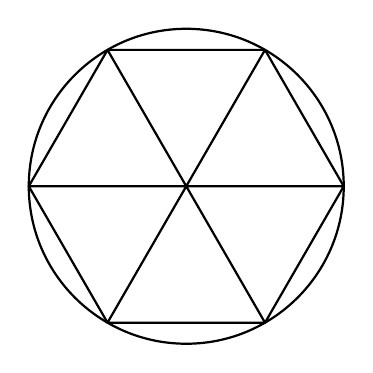
\begin{tikzpicture}[line join = round, line cap = round, scale = 1, thick]
				\def\r{2}
				\foreach \i in {0,60,120,180,240,300}{
					\draw (\i:\r) coordinate (A\i);
				}
				\draw (0,0) circle (2 cm);
				\draw (A0)--(A180) (A60)--(A240) (A120)--(A300) (A0)--(A60)--(A120)--(A180)--(A240)--(A300)--cycle;
			\end{tikzpicture}
		\end{center}
		Vì thiết diện qua trục của hình trụ là hình vuông nên $l=2r$.\\
		Diện tích xung quanh hình trụ $S_{xq}=2\pi rl$ $=2\pi r.2r=36\pi{a^2}$ $\Rightarrow r=3a$\\
		Lăng trụ lục giác đều có đường cao $h=l=6a$\\
		Lục giác đều nội tiếp đường tròn có cạnh bằng bán kính của đường tròn.\\
		Suy ra diện tích lục giác đều $S=6\cdot \dfrac{\left(3a\right)^2\sqrt{3}}{4}$ $=\dfrac{27a^2\sqrt{3}}{2}$ .\\
		Vậy thể tích của lăng trụ lục giác đều là $V=Sh=81\sqrt{3}{a^3}$ .}
\end{ex}

\begin{ex}%[2H2K1-3][Phú Thọ - 2018]
	\immini{
		Cho lăng trụ đứng $ABC.A'{B}'{C}'$ có độ dài cạnh bên bằng $ 2a$, đáy $ ABC$ là tam giác vuông cân tại $ A$, góc giữa $ A{C}'$ và mặt phẳng $\left(BC{C}'{B}'\right)$ bằng $30^{^\circ}$ (tham khảo hình vẽ). Thể tích của khối trụ ngoại tiếp lăng trụ $ ABC.A'{B}'{C}'$ bằng
		\choice
		{$\pi{a^3}$}
		{$ 2\pi{a^3}$}
		{\True $ 4\pi{a^3}$}
		{$ 3\pi{a^3}$}
	}{
		\begin{tikzpicture}[line join=round, line cap=round, scale=1, thick]
			\def\a{3.3} 
			\def\b{1.4}
			\def\h{2.5}
			\def\angle{-55}
			\def\slope{90}
			\path 
			(0,0) coordinate[label=left:$B'$] (A)
			++ (\angle:\b) coordinate[label=below:$A'$] (B)
			(\a,0) coordinate[label=right:$C'$] (C)
			($(A)+(\slope:\h)$) coordinate[label=left:$B$] (A') 
			++(0:\a) coordinate[label=right:$C$] (C') 
			($(B)+(\slope:\h)$) coordinate[label=below left:$A$] (B') 
			;
			\draw[dashed] (A)--(C);
			\draw (A)--(B)--(C) (A')--(B')--(C')--cycle (A)--(A') (B)--(B') (C)--(C') (B')--(C);
		\end{tikzpicture}
	}
	\loigiai{
		\begin{center}
			\begin{tikzpicture}[line join=round, line cap=round, scale=1, thick]
				\def\a{3.3} 
				\def\b{1.4}
				\def\h{2.5}
				\def\angle{-55}
				\def\slope{90}
				\path 
				(0,0) coordinate[label=left:$B'$] (A)
				++ (\angle:\b) coordinate[label=below:$A'$] (B)
				(\a,0) coordinate[label=right:$C'$] (C)
				($(A)+(\slope:\h)$) coordinate[label=left:$B$] (A') 
				++(0:\a) coordinate[label=right:$C$] (C') 
				($(B)+(\slope:\h)$) coordinate[label=below left:$A$] (B') 
				;
				\draw ($(A')!.5!(C')$) coordinate (I) node[above]{$I$};
				\draw[dashed] (A)--(C) (I)--(C);
				\draw (A)--(B)--(C) (A')--(B')--(C')--cycle (A)--(A') (B)--(B') (C)--(C') (B')--(C) (B')--(I);
			\end{tikzpicture}
		\end{center}
		Gọi bán kính của hình trụ là $R$. Gọi $I$ là trung điểm của $BC$. Khi đó $I$ là bán kính một mặt đáy của khối trụ ngoại tiếp lăng trụ $ABC.A'B'C'$.\\
		Ta có $ C{C}'\perp\left(ABC\right)\Rightarrow C{C}'\perp AI$.\\
		Lại có tam giác $ ABC$ là tam giác vuông cân tại $ A$ nên $ AI\perp BC$. Do đó $ AI\perp\left(BC{C}'{B}'\right)$, suy ra $\left(AC',(BCC'B')\right)=\widehat{I{C}'A}=30^\circ$.\\
		Xét tam giác vuông $ AI{C}'$ ta có $ I{C}'=\dfrac{AI}{\tan\widehat{I{C}'A}}$$=R\sqrt{3}$.\\
		Xét tam giác vuông $ CI{C}'$ ta có $ C'I^2=IC^2+C'C^2\Leftrightarrow 3R^2=R^2+4a^2\Rightarrow R=a\sqrt{2}$.\\
		Thể tích khối trụ ngoại tiếp lăng trụ $ ABC.A'{B}'{C}'$ là $ V=\pi{R^2}h$$=4\pi{a^3}$.}
\end{ex}

\begin{ex}%[2H2K1-1][Chuyên Lương Văn Chánh - Phú Yên - 2018]
	\immini{Cho hình trụ $(T)$ có $(C)$ và $\left(C'\right)$ là hai đường tròn đáy nội tiếp hai mặt đối diện của một hình lập phương. Biết rằng, trong tam giác cong tạo bởi đường tròn $(C)$ và hình vuông ngoại tiếp của $(C)$ có một hình chữ nhật kích thước $a\times 2a$ (như hình vẽ). Tính thể tích $V$ của khối trụ $(T)$ theo $a$.
		\choice
		{$\dfrac{100\pi{a^3}}{3}$}
		{\True $250\pi{a^3}$}
		{$\dfrac{250\pi{a^3}}{3}$}
		{$100\pi{a^3}$}
	}{
		\begin{tikzpicture}[line join = round, line cap = round, scale = 1, thick]
			\pgfmathsetmacro\a{0.4}
			\draw (0,0) circle ({5*\a});
			\draw (-5*\a, -5*\a) rectangle (5*\a, 5*\a) (2.4*\a, 3*\a) node{$(C)$};
			\filldraw[pattern=north east lines] (-3*\a, 4*\a) rectangle (-5*\a, 5*\a);
		\end{tikzpicture}
	}
	\loigiai{
		\begin{center}
			\begin{tikzpicture}[line join = round, line cap = round, scale = 1, thick]
				\pgfmathsetmacro\a{0.4}
				\draw (0,0) coordinate (O) node[below right]{$O$} circle ({5*\a});
				\draw (-5*\a, -5*\a) rectangle (5*\a, 5*\a);
				\filldraw[pattern=north east lines] (-3*\a, 4*\a) coordinate (I) node[below left, fill=white]{$I$} rectangle (-5*\a, 5*\a);
				\draw (0, 4*\a) coordinate (H) node[right]{$H$} (-3*\a,0) coordinate (K) node[below]{$K$};
				\draw (-5*\a,0)-|(0,5*\a);
				\draw (H)--(I)--(K) (O)--(I);
			\end{tikzpicture}
		\end{center}
		Gọi $r$ là bán kính đường tròn $(C)$, điều kiện: $r>2a$.\\
		Ký hiệu $O$, $I$, $H$, $K$ là các điểm có vị trí như hình vẽ.\\
		Dễ thấy $OH=r-a$, $OK=r-2a$, $IO=r$. Theo định lý Pitago ta có
		\begin{align*}
			&(r-a)^2+(r-2a)^2=r^2\\
			\Leftrightarrow &\;r^2 - 6ar + 5a^2 = 0\\
			\Leftrightarrow &\;(r-a)(r-5a)=0\\
			\Leftrightarrow &\;\hoac{&r=a\quad (\text{loại vì \(r>2a\))}\\ &r=5a.}
		\end{align*}
		Khi đó khối trụ $(T)$ có bán kính đáy $r=5a$, chiều cao $2r=10a$ nên có thể tích $V=\pi r^2.2r = 250\pi a^3.$
	}
\end{ex}

\begin{ex}%[2H2K1-2][Chuyên Thái Bình - 2018]
	Cho hình trụ có thiết diện qua trục là hình vuông $ ABCD$ cạnh bằng $ 2\sqrt{3}\,\left(\text{cm}\right)$ với $ AB$ là đường kính của đường tròn đáy tâm $ O$. Gọi $ M$ là điểm thuộc cung $\overset\frown{AB}$ của đường tròn đáy sao cho $\widehat{ABM}=60^\circ $. Thể tích của khối tứ diện $ ACDM$ là:
	\choice
	{\True $ V=3\,\left(\text{c}{\text{m}^3}\right)$}
	{$ V=4\,\left(\text{c}{\text{m}^3}\right)$}
	{$ V=6\,\left(\text{c}{\text{m}^3}\right)$}
	{$ V=7\,\left(\text{c}{\text{m}^3}\right)$}
	\loigiai{
		\begin{center}
			\begin{tikzpicture}[line join = round, line cap = round, scale = 1, thick]
				\def\h{4}
				\def\angle{50}
				\pgfmathsetmacro{\r}{2}
				\draw (0,0) coordinate (J) node[below right]{$O$}
				(0,\h) coordinate (I) node[above left]{$O'$};
				\draw (I) ellipse ({\r} and {\r/3});
				\draw (-\r,0) arc (180:360: {\r}  and {\r/3} );
				\draw[dashed] (\r,0) arc(0:180: {\r}  and {\r/3} );
				\draw (-\r,0)--(-\r,\h) (\r,0)--(\r,\h);
				\draw (I)++(\angle:{\r} and {\r/3}) coordinate (C) node[above right]{$C$} ($(I)!-1!(C)$) coordinate (D) node[below left]{$D$};
				\draw (J)++(\angle:{\r} and {\r/3}) coordinate (B) node[above right]{$B$} ($(J)!-1!(B)$)coordinate (A) node[below left]{$A$};
				\draw ($(J)!.5!(B)$) coordinate (H) node[above]{$H$};
				\draw (J)++(-30:{\r} and {\r/3}) coordinate (M) node[right]{$M$};
				\draw[dashed] (I)--(J) (A)--(B)--(C) (M)--(H) (A)--(M)--(B);
				\draw (C)--(D)--(A);
			\end{tikzpicture}
		\end{center}
		
		Ta có $\triangle MAB$ vuông tại $ M$ có $\widehat{B}=60^\circ $ nên $ MB=\sqrt{3}$, $ MA=3$.\\
		Gọi $ H$ là hình chiếu của $ M$ lên $ AB$, suy ra $ MH\perp\left(ACD\right)$ và $ MH=\dfrac{MB.MA}{AB}=\dfrac{3}{2}.$\\
		Vậy $V_{M.ACD}=\dfrac{1}{3}MH\cdot S_{\triangle ACD}=\dfrac{1}{3}\cdot \dfrac{3}{2}\cdot 6=3\,\left(\text{c}{\text{m}^{\text{3}}}\right).$}
\end{ex}

\begin{ex}%[2H2K1-3][THPT Lục Ngạn - 2018]
	Cho hình lăng trụ tam giác đều $ ABC.A'{B}'{C}'$ có độ dài cạnh đáy bằng $a$, chiều cao là $h$. Tính thể tích $ V$ của khối trụ ngoại tiếp hình lăng trụ.
	\choice
	{$ V=\dfrac{\pi{a^2}h}{9}$}
	{\True $ V=\dfrac{\pi{a^2}h}{3}$}
	{$ V=3\pi{a^2}h$}
	{$ V=\pi{a^2}h$}
	\loigiai{
		\begin{center}
			\begin{tikzpicture}[line join=round, line cap=round, scale=1, thick]
				\def\a{2.5} 
				\def\b{1.3}
				\def\h{2.5}
				\def\angle{-40}
				\def\slope{90}
				\path 
				(0,0) coordinate[label=left:$A$] (A)
				++ (\angle:\b) coordinate[label=below:$B$] (B)
				(\a,0) coordinate[label=right:$C$] (C)
				($(A)+(\slope:\h)$) coordinate[label=left:$A'$] (A') 
				++(0:\a) coordinate[label=right:$C'$] (C') 
				($(B)+(\slope:\h)$) coordinate[label=below left:$B'$] (B') 
				;
				\draw[dashed] (barycentric cs:A=1,B=1,C=1) coordinate (G) node[right]{$G$} --++(0,\h);
				\draw[dashed] (A)--(C);
				\draw (A)--(B)--(C) (A')--(B')--(C')--cycle (A)--(A') (B)--(B') (C)--(C');
			\end{tikzpicture}
		\end{center}
		Gọi $ G$ là trọng tâm của tam giác $ ABC$. Do $ ABC$ là tam giác đều nên $ G$ là tâm đường tròn ngoại tiếp tam giác $ ABC$. Hơn nữa $ AG=\dfrac{2}{3}AM=\dfrac{2}{3}\cdot \dfrac{a\sqrt{3}}{2}=\dfrac{a\sqrt{3}}{3}$.\\
		Vậy thể tích của khối trụ ngoại tiếp hình lăng trụ là $ V=\pi{R^2}h=\dfrac{\pi{a^2}h}{3}$.}
\end{ex}

\begin{ex}%[2H2K1-2][THPT Yên Lạc-2018]
	Cho hình trụ có hai đáy là các hình tròn $(O)$, $\left(O'\right)$ bán kính bằng $ a$, chiều cao hình trụ gấp hai lần bán kính đáy. Các điểm $ A$, $ B$ tương ứng nằm trên hai đường tròn $(O)$, $\left(O'\right)$ sao cho $ AB=a\sqrt{6}.$ Tính thể tích khối tứ diện $ ABO{O}'$ theo $ a$.
	\choice
	{\True $\dfrac{a^3}{3}$}
	{$\dfrac{a^3\sqrt{5}}{3}$}
	{$\dfrac{2a^3}{3}$}
	{$\dfrac{2a^3\sqrt{5}}{3}$}
	\loigiai{
		\begin{center}
			\begin{tikzpicture}[line join = round, line cap = round, scale = 1, thick]
				\def\h{4}
				\pgfmathsetmacro{\r}{2}
				\draw (0,0) coordinate (J) node[right]{$O$}
				(0,\h) coordinate (I) node[right]{$O'$};
				\draw (I) ellipse ({\r} and {\r/3});
				\draw (-\r,0) arc (180:360: {\r}  and {\r/3} );
				\draw[dashed] (\r,0) arc(0:180: {\r}  and {\r/3} );
				\draw (-\r,0)--(-\r,\h) (\r,0)--(\r,\h);
				\draw (I)++(138:{\r} and {\r/3}) coordinate (B) node[above left]{$B$};
				\draw (I)++(-110:{\r} and {\r/3}) coordinate (C) node[below left]{$A'$};
				\draw (J)++(-110:{\r} and {\r/3}) coordinate (A) node[below]{$A$};
				\draw[dashed] (A)--(B);
				\draw[dashed] (I)--(J);
				\draw[dashed] (J)--(A);
				\draw (A)--(C)--(B) (B)--(I)--(C);
			\end{tikzpicture}
		\end{center}
		Ta có $O{O}'=2a$, $A'B=\sqrt{A{B^2}-A{A'^2}}=\sqrt{6a^2-4a^2}=a\sqrt{2}$ .\\
		Do đó $A'{B^2}=O'{B^2}+O'{A'^2}=2a^2$ nên tam giác $O'{A}'B$ vuông cân tại $O'$ hay $O'{A}'\perp {O}'B \Rightarrow OA\perp {O}'B$ .\\
		Khi đó $V_{O{O}'AB}=\dfrac{1}{6}OA\cdot O'B\cdot d\left(OA,O'B\right)\cdot \sin\left(OA,O'B\right) =\dfrac{1}{6}a\cdot a\cdot 2a\cdot \sin 90^\circ=\dfrac{a^3}{3}$.}
\end{ex}
\Closesolutionfile{ans}
\indapan{10}{ans/CD22/Muc_7_8}